\documentclass[letterpaper,10pt,3p,preprint]{elsarticle}

\usepackage{amsmath,amssymb,amsfonts}
\usepackage{mathtools}
\usepackage{bm}
\usepackage{tikz-cd}
\usepackage{graphicx}
\usepackage[hidelinks]{hyperref}

\newcommand{\Nbb}{\mathbb{N}}
\newcommand{\Zbb}{\mathbb{Z}}
\newcommand{\Rbb}{\mathbb{R}}
\newcommand{\Cbb}{\mathbb{C}}
\newcommand{\Ebb}{\mathbb{E}}

\newcommand{\Xcal}{\mathcal{X}}
\newcommand{\Ycal}{\mathcal{Y}}
\newcommand{\Zcal}{\mathcal{Z}}
\newcommand{\Wcal}{\mathcal{W}}
\newcommand{\Pcal}{\mathcal{P}}
\newcommand{\Fcal}{\mathcal{F}}
\newcommand{\Gcal}{\mathcal{G}}

\DeclareMathOperator{\ran}{ran}
\DeclareMathOperator{\tr}{tr}
\DeclareMathOperator{\Id}{Id}
\DeclareMathOperator{\supp}{supp}

\DeclareMathOperator{\proj}{proj}
\DeclareMathOperator{\Proj}{Proj}

\DeclarePairedDelimiterX{\abs}[1]{\lvert}{\rvert}{#1}
\DeclarePairedDelimiterX{\norm}[1]{\lVert}{\rVert}{#1}
\DeclarePairedDelimiterX{\innprod}[2]{\langle}{\rangle}{#1,#2}

\newcommand{\vect}[1]{\underline{#1}}
\newcommand{\matr}[1]{\bm{#1}}

\begin{document}

\begin{frontmatter}

\title{Quantum mechanical closure of partial differential
equations with symmetries}

\author[1]{Chris Vales\corref{cor1}}
\ead{chris.vales@dartmouth.edu}
\author[1]{David C. Freeman}
\ead{david.c.freeman.gr@dartmouth.edu}
\author[1]{Joanna Slawinska}
\ead{joanna.m.slawinska@dartmouth.edu}
\author[1]{Dimitrios Giannakis}
\ead{dimitrios.giannakis@dartmouth.edu}

\cortext[cor1]{Corresponding author.}
\affiliation[1]{organization={Department of Mathematics,
    Dartmouth College},
    city={Hanover},
    state={NH 03755},
    country={USA}}

\begin{abstract}
We develop a framework for the dynamical closure of spatiotemporal
dynamics governed by partial differential equations.
Employing the mathematical framework of quantum
mechanics to embed the original classical dynamics into an infinite
dimensional quantum mechanical system,
we use the space of quantum states to model the unresolved
degrees of freedom of the original dynamics and the framework
of quantum measurement to predict their contributions to the
resolved dynamics.
The embedded dynamics is projected to finite dimension
by a positivity preserving discretization process.
Based on methods from operator valued kernels
and delay embedding, the compressed finite dimensional
representation of the dynamics is invariant under the
spatial symmetries of the original dynamics.
We develop a data driven formulation of the scheme that can be
realized numerically and apply it to a dynamical closure problem
for the shallow water equations.
The results demonstrate that our closure model can accurately
predict the main features of the true dynamics,
including for out of sample initial conditions.
\end{abstract}

\begin{keyword}
dynamical closure\sep parametrization\sep quantum mechanics\sep
kernel methods\sep delay embedding\sep transfer operator\sep
shallow water equations
\end{keyword}

\end{frontmatter}

\section{Introduction}\label{sec:intro}
Complex dynamical systems often encompass degrees of freedom that
evolve over a wide range of temporal and spatial scales with
their evolution depending on different physical regimes.
A challenging problem in such multiscale, multiphysics systems
is trying to include dynamical information for degrees of freedom
that either are too computationally expensive to simulate directly
or depend on fully or partially unknown physical processes
\cite{WE2011}.

The approach employed by \emph{closure} or \emph{parametrization}
methods is to derive surrogate dynamical models that can be used
to approximate the contributions of fine grain degrees of freedom
to the dynamics of coarse grain processes we can simulate
consistently.
Early applications include turbulent flows and climate dynamics
\cite{Tennekes1972,Arakawa1974,Gent1989,Sagaut2006},
but closure methods have since found consequential applications
in a wide range of fields
\cite{WE2007}.
For example, in atmospheric dynamics a technique known as
super-parametrization employs deterministic or stochastic column
models with explicitly resolved cloud microphysics as surrogate
models of small scale moist convection, embedded within the
discretization cells of a coarse atmospheric model
\cite{Grabowski1999,Grooms2013}.
In plasma dynamics there have been efforts to derive models
for subgrid scale processes in fluid models
as well as to derive fluid closures of kinetic models,
incorporating both physical modeling and data driven approaches
\cite{Hammett1990,Joseph2016,JYJi2018,ChMa2020,Wang2020,
Matthews2021,Laperre2022,Shukla2022}.

Related to closure is model reduction, which aims
to derive models of reduced complexity that agree in a prescribed
sense with the original dynamics.
For instance, reduced models can be derived using operator theoretic
methods that attempt to justify the model's physical consistency in a
statistical sense
\cite{Grabert1982,Chorin2000,Chorin2002,Parish2017,KLin2021}
or directly through computational methods
\cite{Hinze2005,Chaturantabut2010,Carlberg2013,Benner2015,
Patera2017,Raissi2019,Bhattacharya2021,Lauzon2024}.

Mathematically, closure methods depend on a separation of the
state space of the original dynamical system into two
components: (1) the resolved degrees of freedom, which represent
the coarse grain processes we can simulate or measure consistently
and with tractable cost;
(2) the unresolved degrees of freedom, which are considered too
complex or expensive to simulate or measure directly.
Once the unresolved degrees of freedom have been identified,
one has to define a surrogate model for their
\emph{fluxes}---namely, their contributions---to the
resolved dynamics.
How to define such a model and whether such a model should
be deterministic or stochastic are active areas of research
that use various mathematical tools to offer alternative
approaches
\cite{Majda2005,Pavliotis2008,WE2011,Berner2017,Ahmed2021}.

One approach toward this problem is defining a surrogate model
as a functional relationship between the resolved and unresolved
degrees of freedom.
In this way, the unresolved variables are determined by a
deterministic function of the resolved variables.
A widespread approach of defining such functions that was
especially popular early on relies on expert knowledge of the
modeled physical process to derive formulas that seek to predict
the averaged fluxes to the resolved variables
\cite{Stensrud2013}.
These formulas typically feature tunable parameters
that are calibrated by analyzing numerical, observational
or experimental data through regression or inference techniques
\cite{Neelin2010,Kondrashov2015,Schneider2017,NChen2019}.
More recently, an alternative data driven approach has emerged
where functional relationships are not derived based on
expert physical reasoning but are discovered from data using
machine learning methods
\cite{Brenowitz2018,Pan2018,Rasp2018,BarSinai2019,
Bolton2019,Raissi2019,Lee2020,Yuval2020,Bhattacharya2021,
Bae2022,Charalampopoulos2022,DQi2022,Bracco2025}.

Modeling the unresolved degrees of freedom by a deterministic
function of the resolved degrees corresponds to a reduction in
the dimension of the full state space of the original dynamics.
Regardless of the complexity of the employed functional
relationship, any dynamical independence the unresolved variables
had has been relinquished.
One important consequence of this reduction in state space
dimension is that the resulting parametrized system may
experience a loss in its ability to produce complex
spatiotemporal behavior such as chaotic dynamics
\cite{Palmer2001}.
If that happens, the developed parametrized system will
inevitably struggle to consistently approximate the original
dynamics.

To prevent the reduction of the full state space to the resolved
state space one can introduce a surrogate state space for the
unresolved degrees of freedom and use that space to model their
contributions to the resolved dynamics.
One such approach has been to use stochastic methods to model the
unresolved degrees of freedom, thereby complementing the resolved
state space with the event space of the introduced stochastic
variables
\cite{Majda1999,Crommelin2008,Pavliotis2008,Chorin2015,Berner2017,
Gottwald2017}.

Independently of whether the unresolved variables are represented
using a deterministic or stochastic framework, the main goal of
closure methods is to construct a surrogate model that can
accurately and consistently approximate the original dynamics.
Additionally, it should do so with a tractable computational
cost and without imposing a strong reduction in the complexity
of the predicted dynamical behavior.
Despite the wide variety of mathematical tools employed,
reduction and closure methods can be studied within a
unified operator theoretic framework.
Often referred to as the Mori-Zwanzig formalism,
the framework uses projection operators to describe
the reduction of fine grain degrees of freedom to coarse
grain ones, resulting in exact governing equations for
the coarse grain variables
\cite{Grabert1982,Chorin2000,Chorin2002,KLin2021}.
The derived governing equations offer useful physical
interpretations of the terms that arise in the projection
process, and can be used to derive error bounds and
consistency proofs for downstream reduced models.

A framework called quantum mechanical closure (QMCl)
\cite{Freeman2024}
has been recently developed which models the unresolved degrees
of freedom as a quantum mechanical system.
This approach can be viewed as a generalization of surrogate
modeling based on stochastic models.
Building on earlier work on quantum mechanical data assimilation
\cite{Giannakis2019pre,Freeman2023},
QMCl encodes statistical information about the unresolved degrees
of freedom in a quantum density operator
\cite{Hall2013,Sakurai2021,Takhtajan2008}
that evolves under the transfer operator of the dynamical system
\cite{Baladi2000}.
The fluxes of the unresolved variables are represented by quantum
observables, while the generation of the required flux terms in the
course of timestepping is carried out using tools from the mathematical
theory of quantum measurement
\cite{Hall2013,Sakurai2021,Takhtajan2008}.
The resulting closure scheme is expressed in terms of
linear operators acting on Hilbert spaces.
This enables automatic positivity preservation
(important for modeling sign definite physical quantities such
as density or temperature)
as well as data driven approximation using kernel integral
operator methods
\cite{Coifman2006,Berry2020,Giannakis2019acha}
with rigorous consistency guarantees in the limit of infinite
training data.
QMCl has thus far been applied to the closure of prototype chaotic
ordinary differential equations such as the Lorenz 63 and
multiscale Lorenz 96 models, where it has shown promising
results for the reconstruction of time correlation functions and
long term statistics of observables.

\subsection{Main results}\label{sec:main-results}
In this work we extend the QMCl framework to the case of spatiotemporal
dynamics governed by partial differential equations.
In the extended framework, information about the unresolved degrees
of freedom is encoded in fields of quantum density operators
which are embedded within the spatial discretization cells of the
coarse model.
This produces a framework that can naturally take advantage of the
spatial structure exhibited by partial differential equations,
such as dynamical symmetries.
More specifically, we employ elements of the
vector valued spectral analysis (VSA) framework introduced in
\cite{Giannakis2019vsa}
to develop a data driven scheme that can effectively and efficiently
model the closure of spatiotemporal dynamics in the presence of
symmetries through the use of invariant basis functions.
The closure framework can be used to derive both deterministic and
stochastic surrogate models; in this work we focus on the
deterministic setting.

The main features of the present work can be summarized as follows.
\begin{enumerate}
\item \emph{Positivity preservation}.
As with the original QMCl work, our framework uses the
noncommutative setting of operator algebras to encode the
original classical dynamics, leading to a closure scheme
that is positivity preserving.
This means that positive flux terms in the original
dynamics are represented by positive operators in
our closure model, producing positive surrogate
flux terms.
Generating surrogate fluxes that preserve the sign of the
original fluxes is a nontrivial task and has important
consequences for the closure of dynamics with sign definite
quantities.
\item \emph{Symmetry factorization}.
Taking advantage of the symmetry factorization properties
of the VSA framework, our dynamical closure scheme rests on
a representation of the dynamics that is invariant under the
actions of the spatial symmetry group of the resolved dynamics.
This enables the formation of a compressed representation
of the original spatiotemporal dynamics, leading to a data driven
realization of our closure scheme that can be applied to
complex dynamics with tractable computational cost.
\item \emph{Computational efficiency}.
In addition to the factorization of spatial symmetries,
we implement the data driven formulation of our scheme in a
way that lowers the cost of its most computationally expensive
operations.
As with the original QMCl and VSA frameworks, our data driven
scheme requires solving an eigenvalue problem for a kernel
matrix.
The dimension of this matrix can be very large, making the
eigenvalue problem one of the most expensive tasks in
our scheme.
To address that we compute a low rank approximation
of the original kernel matrix and use it to solve the
eigenvalue problem with reduced cost
\cite{YChen2024,Vales2025evd}.
\item \emph{Application}. We apply our scheme to a closure
problem for the shallow water equations on a one dimensional
spatial domain.
The shallow water equations are a hyperbolic system of partial
differential equations with important applications in fields
such as water waves modeling and ocean dynamics
\cite{Vallis2017,Whitham1999}.
The results demonstrate that our scheme can effectively capture
and reproduce the main features of the dynamics,
including for out of sample initial conditions.
\end{enumerate}

\subsection{Paper layout}\label{sec:layout}
In Section \ref{sec:problem-statement}
we introduce the closure problem under study.
This is followed by a brief overview of the
original QMCl framework in Section \ref{sec:qmcl}.
In Section \ref{sec:qmcl-pdes} we extend this framework to
the closure of spatiotemporal dynamics.
We present the main features of the extended scheme,
the elements it borrows from the VSA framework,
as well as its data driven realization.
In Section \ref{sec:application} we apply the
extended scheme to a closure problem for the shallow
water equations, present our numerical results
and discuss some aspects of the closure scheme
and future work directions.
This is followed by a brief conclusion in
Section \ref{sec:conclusion}.
Finally, \ref{app:implementation}
provides additional details on the numerical implementation
of the data driven formulation of our closure scheme.

\section{Problem statement}\label{sec:problem-statement}
We consider a dynamical system $\Phi^t\colon X\rightarrow X$,
$t\geq 0$ on a generally infinite dimensional state space $X$
possessing an invariant probability measure $\mu$.
The flow map $\Phi^t$ represents the spatiotemporal dynamics
governed by a partial differential equation on a bounded spatial
domain $S\subset\Rbb^c$ for some $c\in\Nbb$.
As such, elements of state space $X$ are functions on the
domain $S$; more specifically, we consider
$X\subset L^2(S,\nu;\Rbb^d)$ with $d\in\Nbb$ and
$\nu$ denoting the Lebesgue measure on $S$.

We decompose the state space as
$X=\Xcal\times\Ycal$
with $\Xcal$ denoting the state space of the resolved degrees
of freedom of the dynamics
and $\Ycal$ the state space of the unresolved degrees.
We assume that the resolved state space $\Xcal\subset X$
is finite dimensional, a property that arises naturally
in many applications.
For instance many dissipative partial differential equations
give rise to long time dynamics that is confined to a finite
dimensional subset of their state space,
such as an inertial manifold
\cite{Constantin1989,Temam1997}.
In other cases discretization of the differential
operator modeling the considered dynamics also yields a finite
dimensional state space.

We define the Hilbert space of vector valued observables
$H=L^2(X,\mu;H_S)$ with $H_S=L^2(S,\nu_M;\Cbb)$
where $\nu_M$ denotes a restriction of the Lebesgue
measure $\nu$ that will be constructed in Section
\ref{sec:qmcl-pdes-closure}.
Every observable $\vec{f}\in H$ represents a
spatiotemporal pattern of the dynamics, for which every state
$x\in X$ yields a function on the spatial domain
$\vec{f}(x)\in H_S$.

We introduce $d$ real observables
$z_j\in H$, $j\in\{0,\ldots,d-1\}$
which will allow us to include in the resolved dynamics
terms that depend on the unresolved variables.
We refer to the observables $z_j$ as the \emph{flux functions}
and to their generated terms $z_j(x)\in H_S$
for any $x\in X$ as their \emph{fluxes}.
In what follows we use $z=\{z_j\}_{j=0}^{d-1}$
to denote the collection of flux functions.
Based on our decomposition of state space $X$
we define the projected flow maps for the resolved dynamics
$\Phi_\Xcal^t\colon X\to\Xcal$,
$\Phi_\Xcal^t=\proj_\Xcal\circ\Phi^t$
and unresolved dynamics
$\Phi_\Ycal^t\colon X\to\Ycal$,
$\Phi_\Ycal^t=\proj_\Ycal\circ\Phi^t$
where $\proj_A$ denotes the canonical projection onto
a subspace $A\subset X$.
With these definitions in place, the dynamics $\Phi^t$ can
be expressed as
\begin{equation*}
    \Phi^t(\hat{x},y)=\bigl(\Phi^t_\Xcal(\hat{x},z(\hat{x},y)),
        \Phi_\Ycal^t(\hat{x},y)\bigr)
\end{equation*}
with state vector $(\hat{x},y)\in\Xcal\times\Ycal$.

Our goal in this work is to construct surrogate dynamics
$\tilde{\Phi}^t\colon\tilde{X}\rightarrow\tilde{X}$
in a surrogate state space
$\tilde{X}=\Xcal\times\tilde{\Ycal}$
where $\tilde{\Ycal}$ denotes a surrogate unresolved state space.
We introduce a surrogate version of the flux functions
$\tilde{z}_j\colon\tilde{\Ycal}\to H_S$
and denote their collection by $\tilde{z}$.
The surrogate dynamics $\tilde{\Phi}^t$ can now be
expressed as
\begin{equation}\label{eq:surr-dyn-decomposition}
    \tilde{\Phi}^t(\hat{x},\tilde{y})=
        \bigl(\tilde{\Phi}_\Xcal^t(\hat{x},\tilde{z}(\tilde{y})),
        \tilde{\Phi}_\Ycal^t(\hat{x},\tilde{y})\bigr)
\end{equation}
with state vector
$(\hat{x},\tilde{y})\in\Xcal\times\tilde{\Ycal}$,
surrogate resolved dynamics
$\tilde{\Phi}_\Xcal^t\colon\tilde{X}\to\Xcal$,
$\tilde{\Phi}_\Xcal^t=\proj_\Xcal\circ\tilde{\Phi}$
and surrogate unresolved dynamics
$\tilde{\Phi}_\Ycal^t\colon\tilde{X}\to\tilde{\Ycal}$,
$\tilde{\Phi}_\Ycal^t=\proj_{\tilde{\Ycal}}\circ\tilde{\Phi}$.
To build the surrogate dynamics map $\tilde{\Phi}^t$ we need to
define the surrogate space $\tilde{\Ycal}$,
the surrogate flux functions $\tilde{z}_j$
and the surrogate dynamics
$\tilde{\Phi}_\Xcal^t$ and $\tilde{\Phi}_\Ycal^t$.

We are particularly interested in systems with dynamical symmetries.
For this reason we assume that there exists a symmetry group $G$
acting on the spatial domain $S$ with a continuous nontrivial
left action
$\Gamma_{S,g}\colon S\rightarrow S$, $g\in G$
which preserves the null sets of measure $\nu$.
The actions $\Gamma_{S,g}$ induce the actions on state space
$\Gamma_{X,g}\colon X\rightarrow X$,
$\Gamma_{X,g}(x)=x\circ\Gamma_{S,g}^{-1}$, $g\in G$.
The actions of group $G$ on $X$ represent dynamical symmetries
of the dynamics $\Phi^t$; namely, we assume the following
equivariance property
\begin{equation*}
    \Gamma_{X,g}\circ\Phi^t=\Phi^t\circ\Gamma_{X,g}
\end{equation*}
for all $t\geq 0$ and $g\in G$.
In such situations we seek to leverage the dynamical symmetries
to reduce training data requirements and the overall dimension
of our surrogate models.

\section{Quantum mechanical closure framework}\label{sec:qmcl}
In this section we provide a brief overview of QMCl as it has
been developed in
\cite{Giannakis2019pre,Freeman2023,Freeman2024},
which is concerned with the closure of dynamics governed
by ordinary differential equations.
The core of the QMCl framework consists of two steps:
(1) embedding the classical dynamics into an infinite dimensional
quantum mechanical system;
(2) projecting the infinite dimensional system to a finite
dimensional subsystem.
The infinite dimensional embedding of the classical dynamics is
treated in Section \ref{sec:qmcl-infinite}.
In Section \ref{sec:qmcl-finite} we present the process used
to project the embedded dynamics to a finite dimensional
subsystem and derive a closure model.

In the description of QMCl provided below we
omit some of the details required for its precise description
and implementation.
A detailed treatment of the scheme, including its data driven realization,
will be given in the following sections once we extend it to the
closure of dynamics governed by partial differential equations.
A detailed analysis of QMCl as presented below can be found in
\cite{Giannakis2019pre,Freeman2023,Freeman2024}.

\subsection{Infinite dimensional embedding}\label{sec:qmcl-infinite}
To build the quantum mechanical closure framework we start by embedding
the classical dynamics on state space $X$ into a quantum mechanical
system on the infinite dimensional Hilbert space
$H=L^2(X,\mu;\Cbb)$.
This involves embedding observables (functions of state) and
probability densities, as well as the evolution of said densities under
the dynamics and their bayesian conditioning.

In the following we denote by $B(H)$ the space of bounded linear
operators on Hilbert space $H$.
We write $Q(H)$ to denote the space of quantum states on $H$
which are positive, trace class operators of unit trace.
We use the term positive operator to describe a selfadjoint
operator with nonnegative spectrum.
Quantum states are also referred to as quantum density operators,
and can be thought of as playing an analogous role to probability
densities in classical statistics.
In this work we mainly use pure quantum states,
which are rank-1 quantum density operators and are
equivalent to projections along a unit vector
\cite{Hall2013,Sakurai2021,Takhtajan2008}.

Every classical observable
$f\in L^\infty(X,\mu;\Rbb)\subset H$
is mapped to a selfadjoint multiplication operator
$A_f\in B(H)$, $A_fg=fg$ for all $g\in H$
referred to as a quantum observable.
Additionally, every classical probability density
$p\in L^1(X,\mu;\Rbb)$, $\sqrt{p}\in H$
is mapped to the quantum density operator
$\rho_p\in Q(H)$,
$\rho_p=\innprod{\sqrt{p}}{\cdot}\sqrt{p}$
representing a pure quantum state.
The expected value of observable $A\in B(H)$
when the quantum system is in state $\rho\in Q(H)$
is given by
$\Ebb_\rho A=\tr(\rho A)\in\Rbb$
which is connected to the theory of quantum measurement
\cite{Hall2013,Sakurai2021,Takhtajan2008}.

We define the surrogate unresolved state space
$\tilde{\Ycal}=Q(H)$
and use a quantum state $\rho\in Q(H)$
to model the state of the unresolved degrees of freedom
of the dynamics.
In addition, we define the operators
$A_j\in B(H)$, $j\in\{0,\ldots, d-1\}$
to model $d$ observables of the system's unresolved state,
which are constructed by mapping the true flux functions
$z_j\in H$ to multiplication operators.
With these definitions in place we introduce the surrogate
flux functions
$\tilde{z}_j\colon Q(H)\rightarrow\Rbb$,
$j\in\{0,\ldots,d-1\}$
with action
\begin{equation*}
    \tilde{z}_j(\rho)=\Ebb_\rho(A_j)=\tr(\rho A_j).
\end{equation*}
In other words we use the space of quantum states
$\tilde{\Ycal}=Q(H)$
to model the unresolved degrees of freedom of the dynamics
and the framework of quantum measurement to compute their
fluxes.

In addition to evaluating the required flux terms we need to be
able to evolve a quantum state under the system's dynamics
and condition it based on observed dynamical behavior.
In the classical case, the square root of probability densities
$\sqrt{p}\in H$
evolves according to the unitary group of transfer operators
$P^t\colon H\to H$,
$P^t\sqrt{p}=\sqrt{p}\circ\Phi^{-t}$ with $t\geq 0$.
Accordingly, the evolution of quantum states $\rho\in Q(H)$
is governed by the induced transfer operator
$\mathcal{P}^t\colon Q(H)\to Q(H)$,
$\mathcal{P}^t\rho=P^t\rho P^{-t}$.
In analogy to bayesian conditioning of classical probability
densities, we can condition a quantum state $\rho\in Q(H)$
using a quantum effect operator $e\in B(H)$, $0\leq e\leq\Id$
\begin{equation}\label{eq:quantum-bayes}
    \rho|_e=\frac{\sqrt{e}\rho\sqrt{e}}{\Ebb_\rho e}
\end{equation}
where $\sqrt{e}$ denotes the positive square root of $e$.
The above equation can be interpreted as the quantum
analogue of the classical Bayes rule
\cite{Freeman2024}.

A quantum effect operator can be thought of as the quantum analogue
of an indicator function used in classical probability to
represent an event, namely a set in the event space.
For instance, for a given set $F\subset X$ we can build the
indicator function $1_F\in H$ taking the value one on $F$
and zero elsewhere.
The quantum effect operator $e_F\in B(H)$ can then be defined
as multiplication by $1_F$, namely
$e_Ff=1_Ff$ for all $f\in H$.

\subsection{Closure modeling}\label{sec:qmcl-finite}
We build a finite dimensional subspace $H^L\subset H$
using the leading $L$ elements of an orthonormal basis
$\{\phi_\ell\}_{\ell=0}^\infty$ of $H$.
To obtain such a basis we define a positive kernel
integral operator $K\colon H\to H$
\begin{equation*}
    Kf=\int_X\kappa(\cdot,x)f(x)\,d\mu(x)
\end{equation*}
using a positive, symmetric and uniformly continuous
kernel function
$\kappa\in C_b(X\times X;\Rbb)\cap L^2(X\times X,\mu\times\mu;\Rbb)$
where $C_b$ denotes the space of bounded continuous functions.
Operator $K$ is compact and selfadjoint, so its eigenfunctions
form an orthonormal basis of $H$;
we write $K\phi_\ell=\lambda_\ell\phi_\ell$
where the eigenvalues $\lambda_\ell$
are nonnegative and ordered in decreasing order.
We define $H^L$ as the linear span of the leading $L$ eigenfunctions
of operator $K$.
Having built $H^L$ we project operators acting on $H$ to
operators acting on $H^L$;
that is, $A\in B(H)$ is approximated by $A_L=\proj_LA\proj_L$ where
$\proj_L\in B(H)$ is the orthogonal projection onto $H^L$.
This is done for all operators needed for the quantum mechanical
embedding of the original classical dynamics.

As explained earlier, to build our closure scheme we set
$\tilde{\Ycal}=Q(H^L)$
and use quantum states to model the unresolved degrees of freedom
of the surrogate dynamics $\tilde{\Phi}^t$ from
\eqref{eq:surr-dyn-decomposition}.
We now describe the calculation of the fluxes needed for evolving the
resolved state under $\tilde{\Phi}_\Xcal^t$,
and the surrogate map $\tilde{\Phi}_\Ycal^t$
used to evolve the quantum state representing the unresolved state.
To do so, we use a discrete time version of the above flow maps,
denoting them by $\tilde{\Phi}_\Xcal^{n\Delta t}$
and $\tilde{\Phi}_\Ycal^{n\Delta t}$
with $n\in\Nbb$ and timestep $\Delta t>0$.

Given the resolved system state
$\hat{x}_n\in\Xcal$ at time $t_n=n\Delta t$
we use a quantum state $\rho_n\in Q(H^L)$
to represent the unresolved state and $d$ quantum observables
$A_j\in B(H^L)$, $j\in\{0,\ldots,d-1\}$.
Each observable $A_j$ is a projected multiplication operator
defined using the corresponding true flux function
$z_j\in H$.
We seek to compute state
$\hat{x}_{n+1}=\tilde{\Phi}_\Xcal(\hat{x}_n,
\tilde{z}(\rho_n))$
using the collection of surrogate flux functions
$\tilde{z}=\{\tilde{z}_j\}_{j=0}^{d-1}$
with $\tilde{z}_j\colon Q(H^L)\to\Rbb$.
Each surrogate flux term $\tilde{z}_j(\rho_n)$
is computed as the expectation value of observable
$A_j$ with respect to quantum state $\rho_n$
\begin{equation*}
    \tilde{z}_j(\rho_n)=\Ebb_{\rho_n}(A_j)=\tr{(\rho_nA_j)}.
\end{equation*}
The resolved state is then updated by
$\hat{x}_{n+1}=\tilde{\Phi}_\Xcal^{\Delta t}(\hat{x}_n,
\tilde{z}(\rho_n))$.

Next we define the surrogate unresolved dynamics map
$\tilde{\Phi}_\Ycal^{\Delta t}$
used to update the quantum state
$\rho_{n+1}=\tilde{\Phi}_\Ycal^{\Delta t}(\hat{x}_n,\rho_n)$.
The quantum state update consists of two steps, a prediction and a
correction step.
Given the current quantum state $\rho_n$ we first use the
projected transfer operator
$\Pcal^L\colon Q(H^L)\rightarrow Q(H^L)$
to compute the prior state
\begin{equation*}
    \rho_{n+1}'=\frac{\Pcal^L\rho_n}
        {\tr{(\Pcal^L\rho_n)}}.
\end{equation*}
Renormalizing the quantum state after acting with $\Pcal^L$
is required because the projected operator $\Pcal^L$
is generally not unitary.
The mapping $\rho_n\mapsto\rho_{n+1}'$ corresponds to the prediction step.
The correction step involves using the updated resolved state
$\hat{x}_{n+1}$ to update our prediction $\rho_{n+1}'$.
To do so, we use state $\hat{x}_{n+1}$ to build a quantum
effect operator $e_{n+1}\in B(H^L)$;
we refer to the mapping $\hat{x}_{n+1}\mapsto e_{n+1}$ as the
\emph{feature map}.
Using the quantum Bayes rule \eqref{eq:quantum-bayes} we condition
the prior state $\rho_{n+1}'$ to compute the posterior state
\begin{equation*}
    \rho_{n+1}=\rho_{n+1}'|_{e_{n+1}}=
        \frac{\sqrt{e_{n+1}}\rho_{n+1}'\sqrt{e_{n+1}}}
        {\tr{(\sqrt{e_{n+1}}\rho_{n+1}'\sqrt{e_{n+1}}})}.
\end{equation*}
The above two steps make up the surrogate unresolved dynamics
$\tilde{\Phi}_\Ycal^{\Delta t}$.
Although not unitary, operator $\Pcal^L$ is trace nonincreasing
which means that it can be interpreted as governing the evolution
of an open quantum system $H^L\subset H$.
Under this light, the reduction of $\tr(\rho)$ when acting with
$\Pcal^L$ can be viewed as decoherence or leakage of density
due to interaction with the environment
\cite{Hall2013,Sakurai2021,Takhtajan2008}.

The QMCl closure framework as developed above can be summarized
in the following diagram, which depicts the evolution of the
built surrogate dynamical system for one timestep
\cite{Freeman2024}.
\begin{equation*}
\begin{tikzcd}[column sep=huge, row sep=large]
    \hat{x}_n\arrow[r,"\tilde{\Phi}_\Xcal^{\Delta t}"]
        &\hat{x}_{n+1}\arrow[r,"\Id"]\arrow[rd,"e_{i+1}"] &\hat{x}_{n+1}\\
    \rho_n\arrow[ru,"\tilde{z}(\rho_n)"]\arrow[r,"\Pcal^L"']
        &\rho_{n+1}'\arrow[r,"\text{Bayes}"'] &\rho_{n+1}
\end{tikzcd}
\end{equation*}
In the diagram $\Id$ denotes the identity map.

\section{Closure of partial differential equations}\label{sec:qmcl-pdes}
In this section we extend the QMCl scheme to the case of
spatiotemporal dynamics governed by partial differential equations.
One of the distinguishing features of the extended scheme is the
appropriate handling of dynamical symmetries.
We develop the extended scheme by pairing QMCl with the
vector valued spectral analysis (VSA) framework
\cite{Giannakis2019vsa},
which combines methods from operator valued kernels and
delay embedding to construct efficient compressed representations
of dynamics in the presence of dynamical symmetries.

In Section \ref{sec:qmcl-pdes-closure}
we define the appropriate Hilbert space $H$ and
describe the process of embedding the classical spatiotemporal
dynamics into a quantum mechanical system in $H$.
In Section \ref{sec:kernel-choice}
we introduce the kernel used to discretize (compress)
the embedded dynamics to a finite dimensional subsystem.
Section \ref{sec:dyn-symmetries}
explores the symmetry invariance property of the derived
eigenfunction basis.
Finally, Sections \ref{sec:data-driven} and \ref{sec:multitrajectory}
present the data driven formulation of the extended QMCl scheme
that can be realized numerically.

\subsection{Closure modeling}\label{sec:qmcl-pdes-closure}
As explained in Section \ref{sec:problem-statement}
we consider spatiotemporal dynamics
$\Phi^t\colon X\rightarrow X$
possessing an invariant probability measure $\mu$
and a generally infinite dimensional state space
$X\subset L^2(S,\nu;\Rbb^d)$
where $S$ denotes a bounded spatial domain.
We assume the state space decomposition $X=\Xcal\times\Ycal$
where $\Xcal$ is the finite dimensional resolved state space
and $\Ycal$ the unresolved state space.

To provide a general definition of the
resolved state space $\Xcal\subset X$
we consider the measure space $(S,\mathcal{A},\nu)$
where $\mathcal{A}$ denotes the Borel $\sigma$-algebra on $S$.
We form the subalgebra $\mathcal{A}_M\subset\mathcal{A}$
generated by a finite collection of $M\in\Nbb$ disjoint subsets
$S_m\subset S$, $m\in\{0,\ldots,M-1\}$
such that $\cup_{m=0}^{M-1}S_m=S$.
Next we define measure $\nu_M$ as the restriction of $\nu$
to $\sigma$-algebra $\mathcal{A}_M$.
The resolved state space is defined as the $dM$-dimensional
subspace $\Xcal=L^2(S,\nu_M;\Rbb^d)\cap X$.
As a Hilbert space, $\Xcal$ is isomorphic to $\Rbb^{dM}$
with a scaled euclidean inner product.
Each subset $S_m\subset S$ used to generate subalgebra $\mathcal{A}_M$
can also be represented by its center point $s_m\in S_m$.
We denote by $S_M=\{s_m\}_{m=0}^{M-1}\subset S$ the collection of
those center points.
Every equivalence class of functions
$\tilde{h}\in L^2(S,\nu_M;\Rbb^d)$
has a piecewise constant representative
$h=\sum_{j=0}^{M-1}\alpha_j 1_{S_j}$
where $1_{S_j}$ denotes the indicator function of set
$S_j\in\{S_m\}_{m=0}^{M-1}$
and $\alpha_j\in\Rbb^d$ the corresponding coefficient.

As our quantum mechanical Hilbert space $H$ we consider
the space of vector valued observables
$H=L^2(X,\mu;H_S)$ with $H_S=L^2(S,\nu_M;\Cbb)$.
Introducing the product state space $\Omega=X\times S$
and measure $\sigma=\mu\times\nu_M$
we define
$H_\Omega=L^2(\Omega,\sigma;\Cbb)$
and note the following Hilbert space isomorphisms
\begin{equation*}
    H\simeq H_X\otimes H_S\simeq H_\Omega,
\end{equation*}
where $H_X=L^2(X,\mu;\Cbb)$.
Namely, for every vector valued observable $\vec{f}\in H$
there is a corresponding complex valued $f\in H_\Omega$
such that for almost every $x\in X$ and $s\in S$
$f(x,\cdot)=\vec{f}(x)\in H_S$ and
$f(x,s)=\vec{f}(x)(s)\in\Cbb$.
The motivation for our choice of space $H$ is our interest
in observables that can effectively capture
\emph{spatiotemporal} dynamics;
that is, patterns of evolution that have both
a temporal dependence $x\in X$ and
a spatial dependence $s\in S$.
Given an observable $\vec{f}\in H$ the map
$t\mapsto\vec{f}(\Phi^t(x))$
represents a spatiotemporal pattern generated by
the dynamics $\Phi^t$
\cite{Giannakis2019vsa}.

The definitions of quantum observables, quantum effects
and the induced transfer operator carry over from
Section \ref{sec:qmcl}
after using the new definition of Hilbert space $H$.
To model the unresolved degrees of freedom we introduce the
surrogate unresolved state space
$\tilde{\Ycal}=L^2(S,\nu_M;B(H))$.
Namely, we use a field of quantum states over $S$,
$\rho\in\tilde{\Ycal}$ with
$\ran{\rho}\subseteq Q(H)\subset B(H)$,
where each quantum state $\rho(s)$ represents the unresolved
degrees of freedom of the dynamics at point $s\in S$
of the spatial domain.
This allows us to compute fluxes that vary over the spatial
domain $S$ for each quantum observable
$A_j\in B(H)$, $j\in\{0,\ldots,d-1\}$.
More specifically, we define the corresponding
$d$ surrogate flux functions
$\tilde{z}_j\colon\tilde{\Ycal}\to H_S$
with action
\begin{equation*}
\tilde{z}_j(\rho)(s)=\tr(\rho(s)A_j)\in\Rbb
\end{equation*}
yielding $d$ flux terms at each spatial point.

Having embedded the original dynamics into an infinite dimensional
quantum system in Hilbert space $H$, we now have to discretize
space $H$ using the eigendecomposition of a kernel integral operator.
We tackle this task in the next section.

\subsection{Choice of kernel}\label{sec:kernel-choice}
To build our closure scheme on $H$ we use data generated from
a dynamical trajectory
$x_n=\Phi^{n\Delta t}(x_0)$ with $x_0\in X$, $n\in\Nbb$
and sampling timestep $\Delta t>0$.
We do not require access to the full state samples $x_n\in X$;
only to the corresponding resolved state samples
$\hat{x}_n=\proj_\mathcal{X}(x_n)\in\mathcal{X}$
and flux samples
$z_j(x_n)\in H_S$, $j\in\{0,\ldots,d-1\}$.
Note that for each $n\in\Nbb$
$\hat{x}_n$ and $z_j(x_n)$ are functions on $S$
with $\hat{x}_n(s)$ and $z_j(x_n)(s)$
denoting their values at point $s\in S$ of the spatial domain.

To discretize the space $H_\Omega\simeq H$ we use the orthonormal
basis generated by the eigenfunctions of a positive kernel
integral operator
$K\colon H_\Omega\rightarrow H_\Omega$
\begin{equation}\label{eq:integral-op}
    Kf=\int_\Omega \kappa(\cdot,\omega)f(\omega)d\sigma(\omega)
\end{equation}
with a positive, symmetric and uniformly continuous kernel
$\kappa\in C_b(\Omega\times\Omega;\Rbb)\cap
L^2(\Omega\times\Omega,\sigma\times\sigma;\Rbb)$.
By forming an operator acting directly on $H_\Omega$ we obtain
eigenfunctions that are generally not of separable, tensor product
form.
This is in contrast to traditional approaches such as the
proper orthogonal decomposition where one builds a basis
for $H_X$ (the temporal space in this context)
and forms its tensor product with a basis for the
spatial space $H_S$ to form a basis for
$H_\Omega\simeq H_X\otimes H_S$
\cite{Aubry1991}.
As we will see below, in the presence of dynamical symmetries
our approach leads to a more compressed finite dimensional
representation of the dynamics on $H$,
meaning that each eigenfunction of operator $K$
as defined above can represent spatiotemporal patterns that
are not expressible as a product of a single pair of temporal
and spatial modes.

To have a kernel function $\kappa$ that relies only on the
sampled information we have access to we employ data space
$\mathcal{W}$ and data map $W\colon\Omega\to\mathcal{W}$.
We introduce the data space kernel
$k\colon\mathcal{W}\times\mathcal{W}\to\Rbb$
and consider $\kappa$ as its pullback
$\kappa(\omega,\omega')=k(W(\omega),W(\omega'))$.
In this work we use a kernel $k$ that acts in delay coordinate space
$\mathcal{W}=\Rbb^Q$
where $Q\in\Nbb$ denotes the number of delays.
As explained below, for each sample
$\omega=(x,s)\in X\times S$
we embed the resolved state component
$(\proj_\Xcal(x),s)\in\Xcal\times S$ into $\Rbb^Q$
by using delays that act locally at spatial point $s\in S$.
This allows us to recover some of the dynamical information lost when
projecting to the resolved component of the state
as well as to factor redundancies introduced in the sampled data
by dynamical symmetries
\cite{Giannakis2019vsa}.

Consider the data map $W_Q\colon\Omega\rightarrow\Rbb^Q$
\begin{equation}\label{eq:data-map}
    W_Q((x,s))=\bigl(\proj_\Xcal(x)(s),\,
        \proj_\Xcal(\Phi^{-\Delta t}(x))(s),\,\ldots,\,
        \proj_\Xcal(\Phi^{-(Q-1)\Delta t}(x))(s)\bigr)
\end{equation}
which corresponds to $S$-pointwise delay embedding of
product state sample $\omega=(x,s)$.
Using this map we define the gaussian kernel function
$k\colon\Rbb^Q\times\Rbb^Q\to\Rbb$
\begin{equation}\label{eq:data-kernel}
    k(W_Q(\omega),W_Q(\omega'))=\exp\Bigl(-\frac{1}{\epsilon Q}
        \norm{W_Q(\omega)-W_Q(\omega')}_Q^2\Bigr)
\end{equation}
where $\norm{\cdot}_Q$ denotes the 2-norm in $\Rbb^Q$ and
$\epsilon>0$ is a tunable bandwidth parameter.
The parameter $\epsilon$ can be calibrated using the procedure
developed in \cite{Coifman2008}.
In our numerical experiments we normalize the above kernel to turn it
into a bistochastic kernel.
The bistochastic kernel normalization process and motivation
for using it can be found in
\cite{Coifman2013,Das2021}.

With this choice of kernel function we use the eigendecomposition
of operator $K$ from \eqref{eq:integral-op} to build an orthonormal
basis for its range $\ran{K}\subset H_\Omega$.
We then use its $L$ leading eigenfunctions
$\{\phi_\ell\}_{\ell=0}^{L-1}$
to define the finite dimensional subspace
$H_{\Omega}^L$ as their linear span.
Once subspace $H_\Omega^L$ has been formed we proceed to project
all operators involved in QMCl from $B(H_\Omega)$
to $B(H_\Omega^L)$.
The resulting operators in $B(H_\Omega^L)$ can be represented
by $L\times L$ matrices with respect to our basis.
This process will be developed in Section
\ref{sec:data-driven}
along with the data driven realization of the extended
closure scheme.

In the next section we describe the properties of the subspace
$\ran{K}\subset H_\Omega$ obtained through the
eigendecomposition of $K$.

\subsection{Dynamical symmetries}\label{sec:dyn-symmetries}
We consider a symmetry group $G$ acting on the spatial domain $S$
by a continuous left action
$\Gamma_{S,g}\colon S\rightarrow S$, $g\in G$.
As explained in Section \ref{sec:problem-statement}
we assume that the dynamics $\Phi^t$ is equivariant under
the actions of $G$
\begin{equation*}
    \Gamma_{X,g}\circ\Phi^t=\Phi^t\circ\Gamma_{X,g}
\end{equation*}
for all $t\geq 0$ and $g\in G$, where
$\Gamma_{X,g}(x)=x\circ\Gamma_{S,g}^{-1}$
denotes the group's induced action on state space $X$.
Every action $\Gamma_{X,g}$ represents a dynamical symmetry
of the dynamics $\Phi^t$.

We consider the decomposition of dynamics
$\Phi^t$ into its resolved $\Phi_\Xcal^t$ and unresolved
$\Phi_\Ycal^t$ components.
In general, the coarsening process used to derive the resolved
dynamics from the original may lead to loss of some of the
original symmetries.
Accordingly, we focus on a subgroup $\Gcal\subseteq G$
that corresponds to the set of symmetries obeyed by the
resolved dynamics $\Phi_\Xcal^t$.
We define the induced action
$\Gamma_{\Xcal,g}\colon\Xcal\rightarrow \Xcal$,
$\Gamma_{\Xcal,g}=\proj_\Xcal\circ\Gamma_{X,g}$, $g\in \Gcal$
and assume that the resolved dynamics $\Phi_\Xcal^t$
is equivariant under the appropriate actions of $\Gcal$
\begin{equation}\label{eq:res-dyn-equivariance}
    \Gamma_{\Xcal,g}\circ\Phi_\Xcal^t=\Phi_\Xcal^t\circ\Gamma_{X,g}
\end{equation}
for all $t\geq 0$ and $g\in \Gcal$.
In addition, we assume that the resolved dynamics is derived
in such a way that the true flux functions $z_j\in H$ satisfy the
analogous equivariance property
\begin{equation*}
    \Gamma_{z,g}\circ z_j=z_j\circ\Gamma_{X,g}
\end{equation*}
for all $g\in\Gcal$ and $j\in\{0,\ldots,d-1\}$
with induced action
$\Gamma_{z,g}\colon H_S\to H_S$.
From now on we focus on subgroup $\Gcal$ and equivariance property
\eqref{eq:res-dyn-equivariance}.
As explained below, our choice of kernel naturally exploits this equivariance
property to bestow an analogous invariance property on the eigenfunctions of
the kernel integral operator.

Under the action of data map $W_Q$ from \eqref{eq:data-map}
the product space $\Omega$ can be viewed as a topological fiber
bundle $(\Omega,B_Q,W_Q)$,
where $\Omega$ is the total space,
$B_Q=W_Q(\Omega)$ the base space and
$W_Q\colon\Omega\rightarrow B_Q$ the continuous projection map.
The fibers are equivalence classes
$[\omega]_Q=W_Q^{-1}(b)\subseteq\Omega$, $b\in B_Q$
defined as the set of values on which $W_Q$ is constant.
For our choice of projection map $W_Q$ each fiber consists of
points in $\Omega$ whose resolved dynamical evolution over $Q$
delays is identical.

Using the group action
$\Gamma_{\Omega,g}\colon\Omega\rightarrow\Omega$,
$\Gamma_{\Omega,g}=\Gamma_{X,g}\otimes\Gamma_{S,g}$
we define the $\Gcal$-orbit of $\omega\in\Omega$ as the set
$\Gamma_\Omega(\omega)=\{\Gamma_{\Omega,g}(\omega)\colon g\in \Gcal\}$.
As shown in \cite{Giannakis2019vsa},
$\Gamma_\Omega(\omega)\subseteq [\omega]_Q$ for all $\omega\in\Omega$;
that is, every fiber $[\omega]_Q$ contains the symmetric transformations
of $\omega$ induced by group $\Gcal$.

Because kernel function $\kappa$ in \eqref{eq:integral-op}
acts by composition with the projection map $W_Q$,
$\kappa=k\circ(W_Q\times W_Q)$,
it is constant on the $[\cdot]_Q$ fibers by construction.
As a result, every function $f\in\ran{K}$ is constant on the fibers;
namely, $f(\omega')=f(\omega)$ for all $\omega'\in [\omega]_Q$.
Given that the $\Gcal$-orbits
$\Gamma_\Omega(\omega)\subseteq [\omega]_Q$
for all $\omega\in\Omega$,
it follows that functions $f\in\ran{K}$
satisfy the invariance property
\begin{equation}\label{eq:G-invariance}
    f\circ\Gamma_{\Omega,g}=f
\end{equation}
for all $g\in\Gcal$.
In particular this implies that all eigenfunctions of integral operator
$K$ corresponding to nonzero eigenvalues satisfy this property as well.
Combined with the fact that all $f\in\ran{K}$ are continuous by
the uniform continuity of $\kappa$,
we conclude that $\ran{K}$ consists entirely of continuous functions
that are constant on the fibers $[\cdot]_Q$.

As a result of \eqref{eq:G-invariance},
by using the eigenfunctions of $K$ corresponding to
nonzero eigenvalues we derive a basis of $\ran{K}$ that is
invariant under the actions of $\Gcal$, instead of
getting multiple ``copies'' of the same underlying functions
generated by the action of different $g\in \Gcal$.
Most importantly for our purposes, this means that fewer eigenfunctions
are needed to represent complex spatiotemporal dynamics,
thereby producing a more efficient compression of the dynamics
from $H_\Omega$ to subspace $H_\Omega^L$
\cite{Giannakis2019vsa}.

\subsection{Data driven formulation}\label{sec:data-driven}
In this section we use the framework developed in the
previous sections to define a data driven closure scheme that
can be realized numerically.
We first establish the data driven formulation using one
dynamical trajectory to generate our training data.
In the next section we extend this to the case of
training data consisting of multiple trajectories.

We consider a finite dynamical trajectory of $N\in\Nbb$ samples
$X_N=\{x_n\}_{n=0}^{N-1}\subset X$
with $x_n=\Phi^{n\Delta t}(x_0)$, $x_0\in X$, $\Delta t>0$.
We define the discrete sampling measure
$\mu_N=\sum_{n=0}^{N-1}\delta_{x_n}/N$
and corresponding finite dimensional Hilbert space
$H_{X,N}=L^2(X,\mu_N;\Cbb)$
where functions are represented by their values
on samples $X_N\subset X$.
Combining the above we define the associated product space
$H_{\Omega,N}=L^2(\Omega,\sigma_{N};\Cbb)$
with discrete product measure
$\sigma_N=\mu_N\times\nu_M$.

We assume that the sampling measures $\mu_N$ converge to
the invariant measure $\mu$
in the weak-$*$ topology of Borel probability measures
on $X$ as $N\to\infty$, meaning that
$\lim_{N\to\infty}\int_Xf\,d\mu_N=\int_Xf\,d\mu$
for all $f\in C_b(X)$.
We refer the reader to
\cite{Freeman2023,Freeman2024}
for details on the convergence properties of the QMCl
scheme in the limit of infinite training data
$N\rightarrow\infty$.

As before we do not assume access to the dynamical trajectory
samples $x_n$ but only to the resolved state samples
$\hat{x}_n=\proj_\Xcal(x_n)\in\mathcal{X}$
and flux samples $z_j(x_n)\in H_S$,
$j\in\{0,\ldots,d-1\}$.
We denote the state samples in product form by
$\omega_{nm}=(x_n,s_m)\in\Omega$
with state $x_n\in X_N$
and gridpoint $s_m\in S_M$.

Using the data space kernel $k$ of \eqref{eq:data-kernel}
we define the associated data driven kernel integral operator
$K_N\colon H_{\Omega,N}\rightarrow H_{\Omega,N}$
\begin{equation}\label{eq:data-integral-op}
    K_Nf=\int_\Omega k_w(W_Q(\cdot),W_Q(\omega))
        f(\omega)d\sigma_N(\omega)
    =\frac{1}{NM}\sum_{n=0}^{N-1}\sum_{m=0}^{M-1}
        k_w(W_Q(\cdot),W_Q(\omega_{nm}))f(\omega_{nm}).
\end{equation}
Using the $L$ leading eigenfunctions
$\{\phi_\ell\}_{\ell=0}^{L-1}$ of $K_N$
we construct the $L$-dimensional subspace
$H_{\Omega,N}^L\subset H_{\Omega,N}$
as their linear span.
Computing the $L$ leading eigenfunctions of $K_N$
can become very expensive as the dimension of the product
space $NM$ is increased.
To address that, in our numerical experiments we build
a low rank approximation of the kernel matrix
$\matr{K}_N\in\Rbb^{NM\times NM}$
associated with operator $K_N$ to compute its
eigenfunctions with reduced cost
(Section \ref{sec:numerics}).
In what follows we make use of the orthogonal projection
$\proj_L\colon H_{\Omega,N}\rightarrow H_{\Omega,N}$,
$\ran{\proj_L}=H_{\Omega,N}^L$.
Using $\proj_L$ an operator
$A\in B(H_{\Omega,N})$
can be projected by conjugation
$\Proj_LA=\proj_LA\proj_L\in B(H_{\Omega,N}^L)$.
Note that the latter projection preserves positivity; namely,
$\Proj_LA$ is a positive operator whenever $A$ is positive.

In the data driven scheme quantum observables are selfadjoint
operators in $B(H_{\Omega,N}^L)$.
To construct such an observable $A_j$ we first define
a multiplication operator
$M_f\in B(H_{\Omega,N})$, $M_fg=fg$
for all $g\in H_{\Omega,N}$
where $f(\omega_{nm})=z_j(x_n)(s_m)$
corresponds to the true flux function $z_j$
viewed as a real valued function in $H_{\Omega,N}$.
Orthogonal projection then yields
$A_j=\Proj_LM_f\in B(H_{\Omega,N}^L)$.
Note that $A_j$ is generally no longer a multiplication operator.
Using the orthonormal basis $\{\phi_\ell\}_{\ell=0}^{L-1}$
each operator $A_j\in B(H_{\Omega,N}^L)$
is represented by a matrix $\matr{A}_j\in\Rbb^{L\times L}$
with entries
$A_{j,ik}=\innprod{\phi_i}{A_j\phi_k}_N$.
In this way for any $g\in H_{\Omega,N}^L$ the operation
$A_jg$ is represented by $\matr{A}_j\vect{g}$
with coefficient vector $\vect{g}\in\Rbb^L$,
$g_\ell=\innprod{\phi_\ell}{g}_N$.
Two distinguishing features of the discretization process
employed by QMCL is that it is contractive and
positivity preserving.
The first property means that the surrogate fluxes produced
by operator $A_j$ are bounded in absolute value by the maximum
absolute value of
$z_j\in H_{\Omega,N}$.
The second property means that that if function $z_j$ is sign
definite (positive or negative) then so will be operator $A_j$,
producing surrogate fluxes that agree in sign with the true
fluxes.

Quantum states form a field
$\rho\in L^2(S,\nu_M;B(H_{\Omega,N}^L))$
with one quantum state
$\rho_m=\rho(s_m)\in Q(H_{\Omega,N}^L)\subset B(H_{\Omega,N}^L)$
for each gridpoint $s_m\in S_M$.
In this work we focus on pure quantum states,
namely rank-1 quantum density operators acting as
projections along a given vector.
For a gridpoint $s_m\in S_M$ quantum state $\rho_m$
is constructed as the projection along a real valued function
$h_m\in H_{\Omega,N}^L$,
$\rho_m=\innprod{h_m}{\cdot}_Nh_m$.
As such, we represent each state $\rho_m$
by the coefficient vector
$\vect{\rho}_m\in\Rbb^L$,
$\rho_{m,\ell}=\innprod{\phi_\ell}{h_m}_N$.
This is equivalent to representing $\rho_m$ by the matrix
$\matr{\rho}_m\in\Rbb^{L\times L}$,
$\rho_{m,ik}=\innprod{\phi_i}{\rho_m\phi_k}_N$
but leads to savings in memory and computation.

For each $j\in\{0,\ldots,d-1\}$
the surrogate flux function
$\tilde{z}_j\colon L^2(S,\nu_M;B(H_{\Omega,N}^L))\to H_S$
maps the quantum state field
$\rho\in L^2(S,\nu_M;B(H_{\Omega,N}^L)))$
to the scalar field
$\tilde{z}_j(\rho)\in H_S$
with $\tilde{z}_j(\rho)(s_m)\in\Rbb$
the computed flux at gridpoint $s_m\in S_M$.
More specifically, given $d$ quantum observables
$A_j\in B(H_{\Omega,N}^L)$
and a quantum state field
$\rho\in L^2(S,\nu_M; B(H_{\Omega,N}^L))$
each surrogate flux function $\tilde{z}_j$ acts by
$\tilde{z}_j(\rho)(s_m)=\tr(\rho(s_m)A_j)\in\Rbb$.
Using our basis representation of each $A_j$ by matrix
$\matr{A}_j\in\Rbb^{L\times L}$ and
$\rho(s_m)$ by vector $\vect{\rho}_m\in\Rbb^L$
we have that
$\tilde{z}_j(\rho)(s_m)
=\vect{\rho}_m^\top\matr{A}_j\vect{\rho}_m$.

The evolution of quantum states is governed by the projected
induced transfer operator
$\mathcal{P}_N^L\colon B(H_{\Omega,N}^L)\to B(H_{\Omega,N}^L)$.
Because we work with pure quantum states---represented
by vectors instead of matrices---we are going to form
the projected transfer operator
$P_N^L\colon H_{\Omega,N}^L\to H_{\Omega,N}^L$
instead of $\mathcal{P}_N^L$.
To build $P_N^L$ we define the shift operator
$P_N\colon H_{\Omega,N}\to H_{\Omega,N}$
\begin{equation*}
    P_Nf(\hat{x}_n,s_m)=\begin{cases}
        0& \text{if $n=0$}\\
        f(\hat{x}_{n-1},s_m)& \text{if $1\leq n<N$}.
        \end{cases}
\end{equation*}
After projection we obtain
$P_N^L=\Proj_LP_N$
represented by a matrix
$\matr{P}_N^L\in\Rbb^{L\times L}$,
$(P_N^L)_{ik}=\innprod{\phi_i}{P_N^L\phi_k}_N$.
Given a single quantum state
$\rho_n\in Q(H_{\Omega,N}^L)$
at time $t_n$ with vector representation
$\vect{\rho}_n\in\Rbb^L$
we obtain the updated state $\vect{\rho}_{n+1}$
by
\begin{equation*}
    \vect{\rho}_{n+1}=\frac{\matr{P}_N^L\,\vect{\rho}_n}
        {\norm{\matr{P}_N^L\,\vect{\rho}_n}_2}.
\end{equation*}
The matrix $\matr{P}_N^L$ is in general not unitary,
which is why we renormalize the updated quantum state after applying
$\matr{P}_N^L$.

Next, quantum effects are operators
$e\in B(H_{\Omega,N}^L)$
used to condition quantum states based on a given
state vector $\omega\in\Omega$.
To build effect $e$ from state vector $\omega$ we introduce
the conditioning kernel function
$\kappa_c\colon\Omega\times\Omega\to\Rbb$,
defined as the pullback of kernel
$k_c\colon\Wcal_c\times\Wcal_c\to\Rbb$,
$\kappa_c(\omega,\omega')=k_c(W_c(\omega),W_c(\omega'))$
with conditioning data space $\Wcal_c$
and associated data map $W_c\colon\Omega\to\Wcal_c$.
To define kernel $k_c$ we introduce the data space
$\Wcal_c=\Rbb^J$ with parameter $J\in\Nbb$.
Additionally, we define the neighborhood function
$\mathcal{N}\colon S\to S^J$
which for a given gridpoint $s_m\in S_M$
returns its $J$ nearest neighbors on $S_M$
in a specified order.
For a given gridpoint $s_m\in S_M$ and state vector
$\omega_m=(x,s_m)\in\Omega$
we then define the action of data map
$W_J\colon\Omega\to\Rbb^J$
by
\begin{equation*}
    W_J((x,s_m))=\bigl(
        \proj_\Xcal(x)(\mathcal{N}^{(0)}(s_m)),\,
        \ldots,\,
        \proj_\Xcal(x)(\mathcal{N}^{(J-1)}(s_m))\bigr)
\end{equation*}
where $\mathcal{N}^{(j)}(s_m)$ denotes the $j$th
component of vector $\mathcal{N}(s_m)$.
For example, for a one dimensional grid $S_M$
and odd $J\in\Nbb$ the action of $W_J$
becomes
\begin{equation*}
    W_J((x,s_m))=\bigl(\proj_\Xcal(x)(s_{m-(J-1)/2}),\,
        \ldots,\,\proj_\Xcal(x)(s_m),\,\ldots,\,
        \proj_\Xcal(x)(s_{m+(J-1)/2})\bigr).
\end{equation*}
The kernel $k_c\colon\Rbb^J\times\Rbb^J\to\Rbb$
is then defined as
\begin{equation}\label{eq:data-kernel-cond}
    k_c(W_J(\omega),W_J(\omega'))=
        \exp\bigl(-\frac{1}{\epsilon' J}
        \norm{W_J(\omega)-W_J(\omega')}_J^2\bigr)
\end{equation}
with $\norm{\cdot}_J$ the 2-norm in $\Rbb^J$ and
$\epsilon'>0$ a bandwidth parameter.
Note that the bandwidth parameter $\epsilon'$ is different
from the one introduced earlier in kernel
\eqref{eq:data-kernel};
it can again be selected using the tuning procedure developed in
\cite{Coifman2008}.
In our numerical experiments we employ the above kernel using a
variable bandwidth function; details on the bandwidth function
and an algorithm for computing it can be found in
\cite{Berry2016,Giannakis2019acha}.

For a fixed gridpoint $s_m\in S_M$ and given a
state vector $\omega_m$ and the full training dataset
$\{\omega_{nm}\}_{nm=0}^{NM-1}$,
kernel $\kappa_c$ is used to produce a function
$f_m\in H_{\Omega,N}$,
$f_m(\cdot)=\kappa_c(\omega_m,\cdot)$
leading to multiplication operator $M_{f_m}$
and the desired quantum effect $e_m=\Proj_LM_{f_m}$.
Employing the quantum Bayes rule \eqref{eq:quantum-bayes}
then yields the conditioned quantum state
$\rho(s_m)|_{e_m}$ for gridpoint $s_m$.
Intuitively, function $f_m$ can be thought of as an affinity function
on state space $\Omega$ measuring how ``similar'' the given
state $\omega_m$ is to the states included in our training dataset.
Building operator $e_m$ and conditioning the prior state
$\rho(s_m)$ then yields the posterior state $\rho(s_m)|_{e_m}$
that encodes the state space affinities captured by $f_m$.
We often refer to the mapping $\omega_m\mapsto e_m$ as the
feature map (as in Section \ref{sec:qmcl-finite})
and to $f_m$ as the \emph{feature vector}
produced by kernel $\kappa_c$ from product state vector
$\omega_m$.

With respect to our basis representation of $\rho(s_m)$
by vector $\vect{\rho}_m\in\Rbb^L$
and effect $e_m$ by matrix $\matr{e}_m\in\Rbb^{L\times L}$
the conditioning operation takes the form
\begin{equation*}
    \vect{\rho}_m|_{e_m}=\frac{\sqrt{\matr{e}_m}\vect{\rho}_m}
        {\norm{\sqrt{\matr{e}_m}\vect{\rho}_m}_2}.
\end{equation*}
To avoid having to compute the square root of matrix $\matr{e}_m$
we modify the way we form effect $e_m$.
We use function $f_m^{1/2}\in H_{\Omega,N}$
to form multiplication operator $\tilde{A}_m=M_{f_m}^{1/2}$
and define effect
$\tilde{e}_m=(\Proj_L\tilde{A}_m)^2=(\tilde{A}_m^L)^2$.
Conditioning with respect to $\tilde{e}_m$ now takes the form
\begin{equation*}
    \vect{\rho}_m|_{\tilde{e}_m}
        =\frac{\sqrt{\matr{\tilde{e}}_m}\vect{\rho}_m}
        {\norm{\sqrt{\matr{\tilde{e}}_m}\vect{\rho}_m}_2}
        =\frac{\matr{\tilde{A}}_m^L\vect{\rho}_m}
        {\norm{\matr{\tilde{A}}_m^L\vect{\rho}_m}_2}.
\end{equation*}
Although effects $\tilde{e}_m$ and $e_m$ are generally different,
the two are equal when $L=N$ and thus also share the same
asymptotic limit as $N\rightarrow\infty$
and $L\rightarrow\infty$
\cite{Freeman2024}.

The data map $W_J$ embeds state vector $(x,s_m)\in\Omega$
into $\Rbb^J$ by considering the resolved state values at
gridpoints neighboring $s_m\in S_M$,
mimicking the structure of the stencil used for the spatial
discretization of the considered dynamics.
In this way kernel $k_c$ compares the stencil of points
around $s_m$ to the corresponding stencil of points for
every state included in our training data.
This makes for a stronger affinity condition than comparing values
of states at only a single gridpoint.
For hyperbolic partial differential equations, where the notion of a
local propagation velocity is well defined, using a stencil of values
is analogous to using a time delayed signal.

Because the spatially local value $\omega_m=(x,s_m)$
is compared to every other state vector present in our training data
$\{\omega_{nm}\}_{nm=0}^{NM-1}$
spatial translations of state $x$ are naturally factored during
the conditioning process.
This means that if a spatial translation of state $x$ is present in
our training dataset then the similarity between product state
$\omega_m=(x,s_m)$
and the corresponding value of the spatial translation of state
$x$ will be identified in the conditioning process.
For partial differential equations with spatial translation
symmetry, this means that we do not have to artificially inflate
our training dataset by including all spatial translations of the
sampled states.

\subsection{Multitrajectory data}\label{sec:multitrajectory}
To build the data driven formulation of our scheme we have so far
relied on a single dynamical trajectory
$x_n=\Phi^{n\Delta t}(x_0)$, $x_0\in X$.
In this section we generalize this construction to the case where
our training data consists of multiple trajectories.
We begin by motivating the use of multiple trajectories
before presenting the modifications required in the
theoretical and data driven formulations of the scheme.

Using a single dynamical trajectory is generally sufficient when
considering a dynamical system possessing a unique physical measure,
namely a measure that can be sampled by a set of
initial conditions of positive measure with respect to the
ambient measure \cite{Blank2017}.
These are measures whose sampling can be realized numerically,
with SRB measures being an important example
\cite{LSYoung2002}.
In such systems, a single long trajectory can be used to sample
the physical measure of the dynamics.

Using multiple trajectories as training data is of interest
when considering dynamical systems possessing multiple
physical measures;
for instance, hamiltonian systems or hyperbolic systems with
several competing basins of attraction.
Additionally, using multiple trajectories is necessary in the
forecasting of parameter dependent systems,
where one considers a dynamical system whose qualitative
dynamics changes with respect to a bifurcation parameter.

Finally, even in systems with a unique physical measure,
being able to use multiple trajectories to sample
that measure allows one to consider optimal sampling
strategies.
In designing such a strategy one tries to optimize the sampling
rate with respect to a chosen objective,
instead of relying on the inherent rate provided
by a single dynamical trajectory.

We consider a finite collection of invariant probability
measures $\{\mu_i\}_i$ on $X$ with mutually disjoint supports
where $i\in\{0,\ldots,I-1\}$ and $I\in\Nbb$.
We define the invariant probability measure
$\mu=\sum_{i=0}^{I-1}\mu_i/I$
and form our quantum mechanical Hilbert space
$H_\Omega=L^2(\Omega,\mu\times\nu_M;\Cbb)$.
Denoting $H_{\Omega,i}=L^2(\Omega,\mu_i\times\nu_M;\Cbb)$
it follows that $H_\Omega$ admits the orthogonal decomposition
\begin{equation*}
    H_\Omega\simeq\oplus_{i=0}^{I-1}H_{\Omega,i}
\end{equation*}
where the isomorphism is up to a rescaling of the inner products
of $H_{\Omega,i}$ by the factor $1/I$.


To realize the above construction numerically we assume access
to sampled trajectories $\{x_n^{(i)}\}_{n=0}^{N_i-1}$
of $N_i\in\Nbb$ samples each, where
$i\in\{0,\ldots,I-1\}$ as above.
Similarly to the single trajectory case from
Section \ref{sec:data-driven},
for each trajectory we define the empirical sampling measure
$\mu_{i,N_i}=\sum_{n=0}^{N_i-1}\delta_{x_n^{(i)}}/N_i$
and assume that $\mu_{i,N_i}\to\mu_i$
in the weak-$*$ sense as $N_i\to\infty$.
We also define the empirical measure
$\mu_N=\sum_{i=0}^{I-1}\mu_{i,N_i}/I$
and associated Hilbert space
$H_{\Omega,N}=L^2(\Omega,\mu_N\times\nu_M;\Cbb)$
with $N=\sum_{i=0}^{I-1}N_i$.
By our assumption that the measures $\mu_i$ have mutually disjoint
supports it follows that the sampled trajectories
$\{x_n^{(i)}\}_{n=0}^{N_i-1}$ are also mutually disjoint.
As a result we have the orthogonal decomposition
\begin{equation*}
    H_{\Omega,N}\simeq\oplus_{i=0}^{I-1}H_{\Omega,N_i}
\end{equation*}
with
$H_{\Omega,N_i}=L^2(\Omega,\mu_{i,N_i}\times\nu_M;\Cbb)$.
Each component space $H_{\Omega,N_i}$ is a space of equivalence
classes of functions represented by their values on the samples
of the $i$th trajectory only.
Leveraging the decomposition of $H_{\Omega,N}$
we use the approach described in Section \ref{sec:data-driven}
to build an eigenfunction basis for each component space
$H_{\Omega,N_i}$ separately and use the
$L_i\in\Nbb$ leading eigenfunctions
$\{\phi_\ell^{(i)}\}_{\ell=0}^{L_i-1}$
to form the subspace
$H_{\Omega,N_i}^{L_i}\subset H_{\Omega,N_i}$.
Denoting $L=\sum_{i=0}^{I-1}L_i$
we define the combined space
\begin{equation*}
    H_{\Omega,N}^L=H_{\Omega,N_0}^{L_0}\oplus\cdots\oplus
        H_{\Omega,N_{I-1}}^{L_{I-1}}
\end{equation*}
with the direct sum of the component bases producing a basis
for the combined space $H_{\Omega,N}^L$.


The basis of $H_{\Omega,N}^L$ derived in this way consists of a
total of $L$ elements, each being an eigenfunction of a block diagonal
operator $K_N=K_{N_0}\oplus\ldots\oplus K_{N_{I-1}}$
with kernel integral operators
$K_{N_i}\colon H_{\Omega,N_i}\to H_{\Omega,N_i}$
in its diagonal blocks.
More specifically, each basis vector $\phi_\ell^{(i)}$
represents the values of a function on $N$ samples,
with all of its values being zero except for the block of values
that corresponds to the $N_i$ samples of the $i$th trajectory it
was derived from.
This approach has lower computational cost compared to building
an eigenfunction basis for $H_{\Omega,N}$
by using a single kernel integral operator,
which would require solving an eigenvalue problem for an
$N\times N$ matrix.
However, our approach also requires that each invariant measure
$\mu_i$ is individually adequately sampled,
as opposed to adequate joint sampling of measure $\mu$.
This can potentially limit the number of high quality basis functions
that can be derived from a dataset of fixed size $N$,
for instance if one chooses to use a large number of trajectories
with a small number of samples $N_i$ for each one.


Having derived the basis for space $H_{\Omega,N}^L$
the construction of the rest of the scheme proceeds as in
Section \ref{sec:data-driven}.
The only additional difference is in the definition of the
shift operator $P_N$
where time shifts are now applied only \emph{within} each
trajectory, and the first temporal sample of each trajectory
is mapped to zero.
Namely, we make sure not to shift samples
\emph{across} different trajectories.

After forming our QMCl closure model in $H_{\Omega,N}^L$
our goal is to use it to predict the dynamics of a chosen
dynamical system for out of sample initial conditions;
namely, initial conditions lying outside of the basins of the
measures $\mu_i$ sampled in the training stage.
Thanks to the fact that the feature maps used to form
quantum effects (Section \ref{sec:data-driven})
are not restricted to our training dataset,
our closure scheme can ingest information from the resolved variables
and render estimates of the fluxes even for out of sample data.
Whether these estimates are sufficiently accurate ultimately depends
on whether the kernel used for the conditioning of quantum states can
identify samples of our training dataset whose corresponding flux
evolution is similar to that of out of sample initial conditions.
In the next section we present numerical results offering empirical
evidence that out of sample predictions can indeed be made using
QMCl for the tested dynamical system and family of initial conditions.


\section{Application}\label{sec:application}
The shallow water equations govern the evolution of a fluid when its
vertical length scale can be considered negligible compared to its
horizontal length scale.
The equations are derived from the conservation laws for mass and momentum.
Various forms of the equations have applications in areas such as
ocean fluid dynamics, often incorporating additional terms modeling
the effects of bottom topography and Coriolis force
\cite{Vallis2017,Whitham1999}.

We consider the shallow water equations on the one dimensional spatial
domain $S=[-L_S/2,L_S/2]$ with periodic boundary conditions.
The system of equations governs the evolution of water height
$h(t,\cdot)$ and momentum $q(t,\cdot)=h(t,\cdot)v(t,\cdot)$
with $v(t,\cdot)$ denoting the velocity field and
$t\geq 0$ time.
The scalar fields $h(t,\cdot)$ and $q(t,\cdot)$ are assumed
to take values in a sufficiently regular subset of
$L^2(S,\nu;\Rbb)$ for all $t\geq 0$.
The governing equations read
\begin{equation}\label{eq:swe}
\begin{aligned}
    \partial_th+\partial_sq&=0\\
    \partial_tq+\partial_s(q^2/h+1/2Fr^{-2}h^2)&=0
\end{aligned}
\end{equation}
subject to an appropriate initial condition.
In the above $\partial_t$ and $\partial_s$ denote differentiation
with respect to time and space respectively;
$Fr$ denotes the flow's Froude number, which is a
dimensionless ratio of inertial over gravitational forces.
Using the state variable
$x=(h,q)\in X\subset L^2(S,\nu;\Rbb^2)$
and function
$f(x)=(q,q^2/h+1/2Fr^{-2}h^2)$
we rewrite \eqref{eq:swe} in the compact form
\begin{equation}\label{eq:swe2}
    \partial_tx+\partial_sf(x)=0.
\end{equation}
The dynamics governed by \eqref{eq:swe2} is equivariant under the
actions of the spatial translation group on $S$.

We define the total energy of the fluid as the sum of its kinetic
and potential energies
\begin{equation*}
    E(t)=\frac{1}{2}\int_S\frac{q^2(t,s)}{h(t,s)}\,d\nu(s)
        +\frac{1}{2}Fr^{-2}\int_Sh^2(t,s)\,d\nu(s)
\end{equation*}
for all $t\geq 0$.
If one assumes that the height and velocity fields are differentiable
for all $t\geq 0$, thereby excluding discontinuous solutions,
then the total energy is conserved along solution trajectories,
namely $dE(t)/dt=0$.
In this case the state space can be decomposed into the dynamics
invariant disjoint subsets
\begin{equation*}
    \mathcal{E}_c=\{x\in X\colon E(t)=c\text{ for all $t\geq 0$}\}
\end{equation*}
each one defined as the subset of constant energy $c\geq 0$.

In the formation of discontinuities, the internal energy of
the fluid is increased across a discontinuity, accompanied by an
increase in entropy.
Since the above definition of total energy does not
include internal energy, the total energy is decreased across a
discontinuity \cite{Whitham1999}.
In the present work we consider only differentiable solutions.

\subsection{Discretization}\label{sec:swe-discretization}
We employ a finite volume spatial discretization of
\eqref{eq:swe2}
using a uniform fine grid of $M_f\in\Nbb$ cells with length
$\Delta s=L/M_f$ each, centered at points
$s_m\in S$, $m\in\{0,\ldots,M_f-1\}$.
We denote
$S_f=\{s_m\}_{m=0}^{M_f-1}\subset M$
and
$C_m=[s_m-\Delta s/2,s_m+\Delta s/2]\subset S$,
$m\in\{0,\ldots,M_f-1\}$
where each cell $C_m$ can also be represented by its
center point $s_m\in S_f$.
We define the cell averaged state variable
\begin{equation*}
    x(t,s_m)=\frac{1}{\Delta s}\int_{s_m-\Delta s/2}^{s_m+\Delta s/2}
        x(t,\tilde{s})d\nu(\tilde{s}),\quad s_m\in S_f
\end{equation*}
reusing the same state symbol $x$.
For any $t\geq 0$ function $x(t,\cdot)$ can be represented by
the vector $\vect{x}\in\Rbb^{2M_f}$
with $x_m=x(t,s_m)$, $s_m\in S_f$.

We derive the semidiscretized system of equations governing the
evolution of the state variables
\begin{equation}\label{eq:swe-semi}
    \dot{x}_m=\frac{1}{\Delta s}(F_m-F_{m+1})
\end{equation}
using the local Lax-Friedrichs (LLF) numerical flux
\begin{equation}\label{eq:llf-flux}
    F_m=\frac{1}{2}[f(x_{m-1})+f(x_m)]
        -\frac{\lambda_m}{2}(x_m-x_{m-1})
\end{equation}
with
\begin{equation}\label{eq:llf-wavespeed}
    \lambda_m=\max\,\bigl(\abs{q_{m-1}/h_{m-1}}+Fr^{-1}\sqrt{h_{m-1}},
        \,\abs{q_m/h_m}+Fr^{-1}\sqrt{h_m}\bigr).
\end{equation}
In the above, subscripts denote components of the associated vectors
while $F_m$ denotes the numerical flux at the left face
of cell $C_m$ \cite{LeVeque2002}.
Based on \eqref{eq:llf-flux} and \eqref{eq:llf-wavespeed}
we introduce the notation
\begin{equation*}
    F_m=\Fcal_{LLF}(x_{m-1},x_m)
\end{equation*}
which will be used later on to define the coarse grid fluxes.

We now form a coarse grid and associated coarse variables defined
as local spatial averages of the fine variables $x_m$.
In particular we form $M_c\in\Nbb$ coarse grid cells by merging every
$M_s\in\Nbb$ fine cells; in this way, $M_c=M_f/M_s$ and each coarse
cell has length $\Delta\hat{s}=M_s\Delta s$.
We define the resulting coarse grid
$S_c=\{\hat{s}_m\}_{m=0}^{M_c-1}\subset S$
with cells
$\hat{C}_m=[\hat{s}_m-\Delta\hat{s}/2,
\hat{s}_m+\Delta\hat{s}/2]\subset S$,
$m\in\{0,\ldots,M_c-1\}$.
The coarse grid state variable $\hat{x}$ is formed
using spatial averages over each coarse cell
\begin{equation*}
    \hat{x}(t,s_m)=\frac{1}{M_s}\sum_{j=M_sm}^{M_s(m+1)-1}x_j,
        \quad s_m\in S_c
\end{equation*}
and is represented by the vector
$\vect{\hat{x}}\in\Rbb^{2M_c}$
with $\hat{x}_m=\hat{x}(t,s_m)$, $s_m\in S_c$.
For the evolution of the coarse state variable $\hat{x}$
we derive the system of equations
\begin{equation}\label{eq:swe-semi-coarse}
    \dot{\hat{x}}_m=\frac{1}{\Delta\hat{s}}
        [(\hat{F}_m+G_m)-(\hat{F}_{m+1}+G_{m+1})]
\end{equation}
with coarse grid fluxes
\begin{equation}\label{eq:coarse-flux}
    \hat{F}_m=\mathcal{F}_{LLF}(\hat{x}_{m-1},\hat{x}_m)
\end{equation}
and subgrid fluxes
\begin{equation}\label{eq:subgrid-flux}
    G_m=F_{M_sm}-\hat{F}_m.
\end{equation}
The system \eqref{eq:swe-semi-coarse} is equivariant under the
actions of the discrete group of spatial translations on $S_c$.

By definition, the coarse grid fluxes \eqref{eq:coarse-flux} depend
only on the coarse variables.
On the contrary, the subgrid fluxes \eqref{eq:subgrid-flux} depend
on both the coarse and the original fine variables;
in particular, they depend on the values of $x_m$
in the fine cells that border the interfaces of each coarse cell.
The subgrid fluxes act as antidiffusive corrections to the coarse
grid fluxes, increasing the accuracy of the discretization compared
to one performed entirely on the coarse grid
\cite{Timofeyev2025}.

The temporal discretization of evolution equations
\eqref{eq:swe-semi} and \eqref{eq:swe-semi-coarse}
is carried out using the modified Euler method
(two-stage Runge-Kutta), which has favorable structure
preservation properties for the present problem
\cite{Timofeyev2025}.
In what follows we consider the coarse mesh variables as the resolved
degrees of freedom and the discrete time version of
\eqref{eq:swe-semi-coarse}
as the true resolved dynamics.
For the system to be complete we need to provide a closure model
that can infer the subgrid fluxes $G_m$ from the resolved variables
$\hat{x}_m$, thereby removing the explicit dependence on the
fine mesh variables $x_m$.

\subsection{Closure model}\label{sec:swe-closure}
To define the appropriate state space $X$ for the dynamics
we begin by considering the measure space
$(S,\mathcal{A},\nu)$ where $\mathcal{A}$ denotes
the Borel $\sigma$-algebra on the spatial domain $S$.
We form $\mathcal{A}_f\subset\mathcal{A}$
as the $\sigma$-algebra generated by the disjoint subsets
$C_m\subset S$ that correspond to the fine
discretization cells;
analogously, we form
$\mathcal{A}_c\subset\mathcal{A}$
as the $\sigma$-algebra generated by the coarse
cells $\hat{C}_m\subset S$.
We define measures $\nu_f$ and $\nu_c$ as the restrictions
of $\nu$ to the $\sigma$-algebras
$\mathcal{A}_f$ and $\mathcal{A}_c$
respectively.

The state space of the true spatiotemporal dynamics
\eqref{eq:swe2} is an infinite dimensional Hilbert space
$X\subset L^2(S,\nu;\Rbb^2)$.
To be able to simulate the ``true'' dynamics numerically
we approximate the state space by
$X\subset L^2(S,\nu_f;\Rbb^2)$
where $X$ is now considered as a Hilbert subspace of the space of
$L^2$ functions on the mesh produced by our fine discretization.
Next we define the resolved state space
$\Xcal=L^2(S,\nu_c;\Rbb^2)\cap X$
and decompose the full state space as $X=\Xcal\oplus\Ycal$
with unresolved state space $\Ycal=\Xcal^{\perp}$.
In this way the resolved state space can be considered as a
space of piecewise constant functions, each taking a constant
value on each cell formed by the coarse discretization.
The full dynamics
$\Phi^{n\Delta t}\colon X\to X$
is now given by the discrete time version of
\eqref{eq:swe-semi}
and the resolved dynamics
$\Phi_\Xcal^{n\Delta\hat{t}}\colon X\to\Xcal$
by the discrete time version of
\eqref{eq:swe-semi-coarse}
with $n\in\Nbb$ and timesteps $\Delta t>0$
and $\Delta\hat{t}=M_s\Delta t$.

We define the product state space $\Omega=X\times S$
and associated Hilbert space of observables
$H_{\Omega,N}=L^2(\Omega,\sigma_N;\Cbb)$
with total number of samples $N\in\Nbb$
and measures $\sigma_{N}=\mu_N\times\nu_M$
and $\nu_M=\nu_c$.
For notational consistency with the previous sections,
in the following we denote by $M=M_c$ the number of coarse grid cells
and by $S_M=S_c\subset S$ the set of grid points representing the coarse
grid cells.
We introduce two flux functions
$z_j\in H_{\Omega,N}$, $j\in\{0,1\}$
producing the fluxes for the height and momentum
variables respectively,
denoting their collection by $z=\{z_j\}_{j=0}^1$.
For every state $x\in X$ the fluxes $z_j(x)$ are given
by \eqref{eq:subgrid-flux}.

Using the full dynamics we generate $N$ samples of the resolved state
$\{\hat{x}_n\}_{n=0}^{N-1}$ and fluxes
$\{z(x_n,\cdot)\}_{n=0}^{N-1}$
which will be used as our training data
and may consist of one or more dynamical trajectories.
Each sample $\hat{x}_n$ or $z(x_n,\cdot)$
is represented by a vector in $\Rbb^{2M}$
holding the values corresponding to the height
$h$ and momentum $q$ variables in each coarse grid cell.

To form our closure model we define
the surrogate unresolved state space
$\tilde{\Ycal}=L^2(S,\nu_M;B(H_\Omega))$
and two quantum observables
$A_j\in B(H_{\Omega,N})$, $j\in\{0,1\}$.
Observable $A_0$ will be used to produce the surrogate fluxes
for the height $h$ variables and is formed as multiplication by
the true flux function $z_0$;
analogously, observable $A_1$ will produce the surrogate fluxes
for the momentum $q$ variables and is defined as multiplication
by $z_1$.
With these definitions in place, the surrogate fluxes are
computed using the two surrogate flux functions
$\tilde{z}_j\colon\tilde{\Ycal}\to H_S$
with action
$\tilde{z}_0(\rho)(s_m)=\tr(\rho(s_m)A_0)$
and
$\tilde{z}_1(\rho)(s_m)=\tr(\rho(s_m)A_1)$
where $\rho\in\tilde{\Ycal}$
and $s_m\in S_M$.

In \ref{app:implementation} we explain the sequence of
steps used to build the data driven QMCl scheme and apply
it to predict the dynamics based on a given initial condition.

\subsection{Numerical results}\label{sec:numerics}
We consider the shallow water equations
\eqref{eq:swe2}
on the spatial domain $S=[-25,25]$
with Froude number $Fr=1/\sqrt{2g}$
and $g$ denoting the acceleration of gravity.
We perform the spatial discretization using a fine grid of
$M_f=1920$ cells and the temporal discretization using the
midpoint Euler method and a timestep $\Delta t=0.1\Delta s$
where $\Delta s$ is the length of each fine cell.

\subsubsection*{Training}
We define the one-parameter family of initial conditions
\begin{equation}\label{eq:ic-family}
\begin{aligned}
    h_0(s) &= 1 + 0.3(1-\delta/2)\sin\Bigl(\frac{2\pi}{L_S}
        3.5(1-\delta/2)s+\pi/6\Bigr)\\
    v_0(s) &= 1 + 0.2(1-\delta)\sin\Bigl(\frac{2\pi}{L_S}
        3(1-\delta)s\Bigr)
\end{aligned}
\end{equation}
with $s\in S$, $L_S=50$, parameter $0\leq\delta\leq1$,
$h_0$ the initial condition for height and
$q_0=h_0v_0$ the initial condition for momentum.
The solutions generated by this family of initial conditions
feature a number of wave fronts traveling in different directions
and interacting with one another.
Figures \ref{fig:res01a} and \ref{fig:res02a}
present space-time heatmaps of the solutions that will be used
to test the predictive performance of our closure model.


\begin{figure}[t]
    \centering
    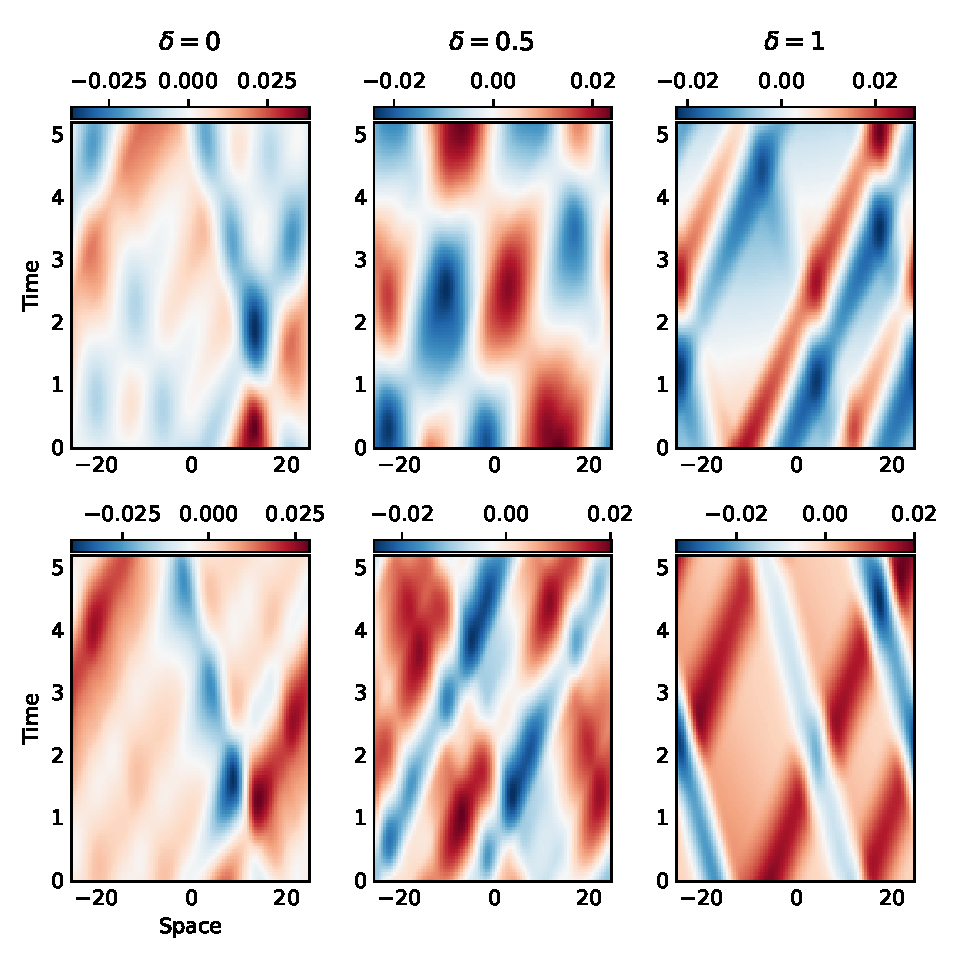
\includegraphics[width=.7\textwidth]{vsabasis.pdf}
    \caption{Space-time heatmaps depicting two eigenfunctions
    $\phi_\ell$ of the kernel integral operator $\matr{K}_N$
    from \eqref{eq:data-integral-op}
    for each of the three trajectories used as our training data.
    The top row shows the third eigenfunction for each of the
    three trajectories; the bottom row the fourth eigenfunction
    for each trajectory.
    From left to right, the first column corresponds to the
    trajectory data obtained for $\delta=0$,
    the second to $\delta=0.5$
    and the third to $\delta=1$.}
    \label{fig:vsa-basis}
\end{figure}

Using the assumptions and methodology introduced
in Section \ref{sec:multitrajectory} for dealing
with multitrajectory training data,
we consider $\mu$ to be the measure generated by
the full dynamics \eqref{eq:swe-semi}
restricted to the family of initial conditions
\eqref{eq:ic-family} for $\delta\in [0,1]$.
To sample this measure we use three trajectories generated
using the values $\delta\in\{0,0.5,1\}$.
For each trajectory we integrate the full dynamics
\eqref{eq:swe-semi}
in time for 12,200 timesteps and then sample the next
3,260 timesteps.
Each sample contains the values of functions $h$ and $q$
on the fine grid.

To derive the resolved state samples that will be used as our
training data, we coarsen the model and sampled data.
By averaging the sampled data over every $M_s=20$ fine cells
we arrive at a coarse grid of $M=96$ cells of length
$\Delta\hat{s}=20\Delta s$ each.
Given that each cell is now $20$ times longer we also increase
the sampling timestep by the same amount to set
$\Delta\hat{t}=20\Delta t$.
From the original 3,260 samples per trajectory generated on the
fine grid we keep every 20th sample, leading to 163 samples
per trajectory.
For each one of those samples we spatially average the solution over
every $20$ cells to derive our resolved state samples,
namely the averaged values of $h$ and $q$ over the coarse grid.
We then derive the subgrid flux training samples using
\eqref{eq:subgrid-flux}.

Using $Q=64$ delays, these samples yield 100 training samples
per trajectory in delay embedded form, adding up to $N=300$
samples in total.
Each resolved state sample consists of $2M=192$ values,
96 for each of the height and momentum variables.
With this training dataset the dimension of the product
Hilbert space $H_{\Omega,N}$ is equal to $NM=28800$.
Employing the approach described in Section \ref{sec:multitrajectory}
we build an orthonormal basis $\{\phi_\ell\}_{\ell=0}^{L-1}$
using a total of $L=6144$ eigenfunctions and define
$H_{\Omega,N}^L$ as their linear span.
Each eigenfunction is represented by a vector in $\Rbb^{NM}$.
Finally, we set $J=5$ to define data map $W_J$ that will be used
for the bayesian conditioning of quantum states.
The data driven realization of the closure model developed
in Section \ref{sec:swe-closure}
will take place in $H_{\Omega,N}^L$.

The number of delays $Q$ was chosen by a combination of
physical reasoning and trial and error
to balance the effectiveness of the derived basis
in representing the true flux samples and the cost associated
with its computation.
A useful rule of thumb is to select a delay window that is
comparable to the timescale of the physical processes of interest.
In our case, we see that the traveling wave fronts interact
approximately every 30 timesteps ($\approx 1.5$ time units)
for the solution in Figure \ref{fig:res01a}
and approximately every 50 timesteps ($\approx 2.5$ time units)
for the solution in Figure \ref{fig:res02a},
with similar results for additional solutions not shown here.
Using $Q=64$ is sufficient to ensure that at least one period
of this interaction is captured in each delay embedded sample.
Additionally, increasing the value of $Q$ further did not lead
to noticeable differences in our results.
The stencil size $J$ used for the conditioning of quantum states
was chosen empirically.
Increasing the value of $J$ further was shown to slightly improve
the performance of the bayesian conditioning operation, but with
an associated increase in computational cost.

To form the orthonormal basis
$\{\phi_\ell\}_{\ell=0}^{L-1}$
we must compute the eigenvectors of an $NM\times NM$
symmetric kernel matrix $\matr{K}_N$ representing the
data driven integral operator
\eqref{eq:data-integral-op}.
To reduce the computational cost of this operation
we perform a partial Cholesky factorization of
$\matr{K}_N$ to approximate it by a lower rank matrix
$\tilde{\matr{K}}_N=\matr{F}\matr{F}^T$
with $\matr{F}\in\Rbb^{NM\times r}$ and $r<NM$.
We perform the factorization using rank parameter
$r=L=6144$ and the randomized algorithm developed in
\cite{YChen2024}.
We then use the approximate kernel matrix to perform its
bistochastic normalization and solve the eigenvalue
problem with reduced cost
\cite{Vales2025evd}.

A selection of the resulting eigenfunctions is presented in
Figure \ref{fig:vsa-basis},
where we show two eigenfunctions for each of the three
trajectories used to build our training dataset.
The shown eigenfunctions exhibit propagating fronts
which resemble the main features of the true state and flux
samples presented in Figures
\ref{fig:res01a} and \ref{fig:res02a}.
More specifically, they are approximately constant on the
characteristic lines of the propagating wave fronts,
as expected from their symmetry invariance property.
Similar features are present in the rest of the eigenfunctions
not shown here.
As explained in Sections
\ref{sec:kernel-choice} and \ref{sec:dyn-symmetries}
the strong dynamic relevance of each eigenfunction is a result
of its spatial symmetry invariance and of
the fact that generally it cannot be represented as the tensor
product of a single pair of spatial and temporal modes.
These properties allow us to compute a compressed representation
of the true dynamics with a moderate number of eigenfunctions,
enhancing the computational efficiency of the resulting closure
scheme.

\subsubsection*{Prediction}
To test the predictive performance of the QMCl scheme we use two
initial conditions obtained from \eqref{eq:ic-family}
for $\delta\in\{0.25,0.75\}$
which are trajectories not included in the training dataset.
After integrating the true dynamics \eqref{eq:swe-semi}
for 12,200 timesteps we spatially average the found solutions
to generate the initial conditions that will be used to initialize
the resolved state in QMCl.
Using those initial conditions we integrate in time the coarse
dynamics \eqref{eq:swe-semi-coarse} using timestep $\Delta\hat{t}$
and the subgrid fluxes predicted by QMCl.
In what follows we present results obtained after integrating for
a total of 120 timesteps while performing bayesian conditioning
of the quantum states every 10 timesteps.

\begin{figure}[t!]
    \centering
    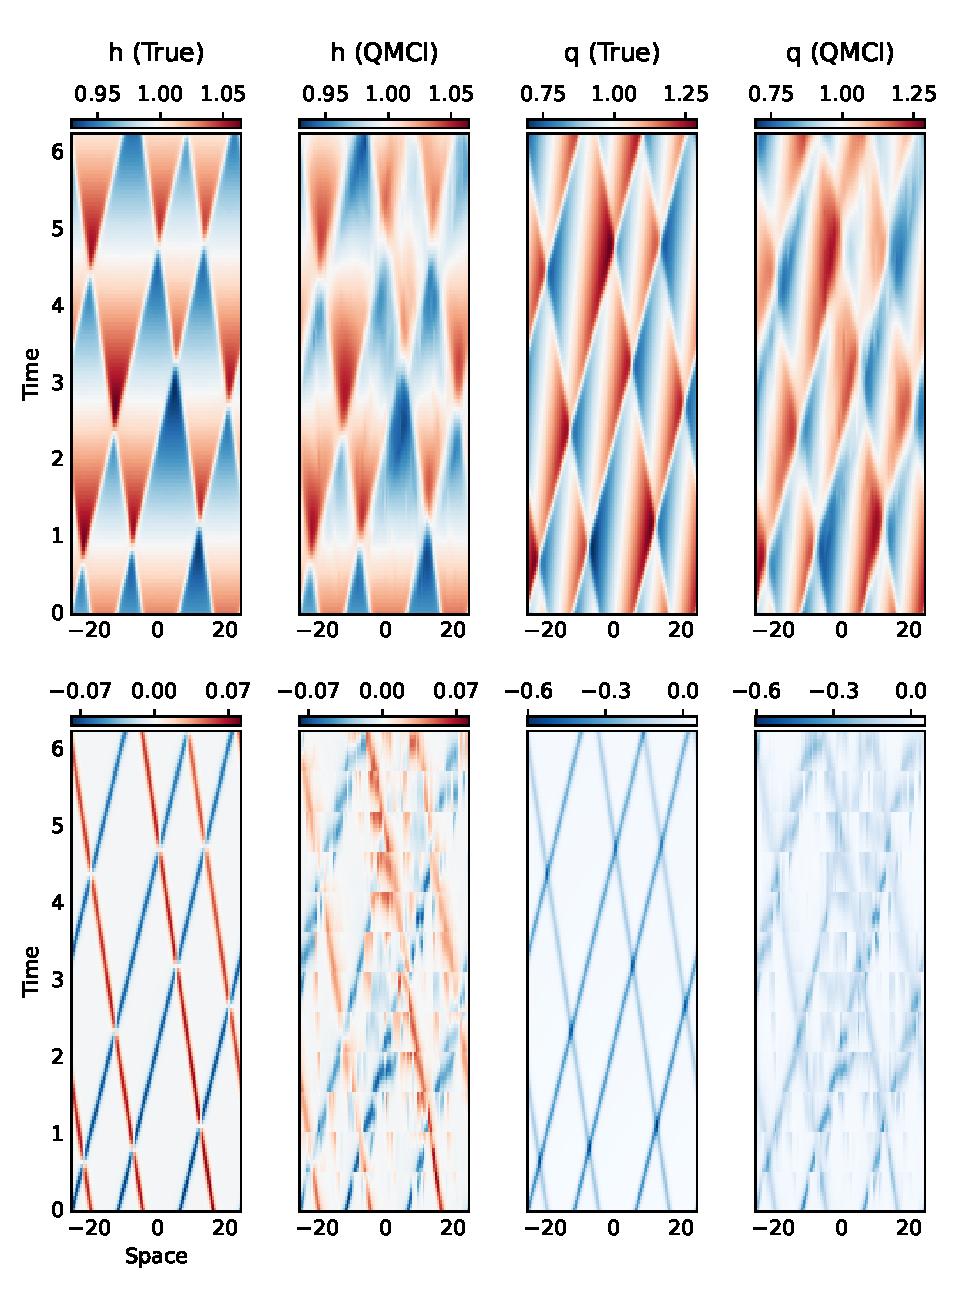
\includegraphics[width=.7\textwidth]{res01a.pdf}
    \caption{Space-time heatmaps for the trajectory with $\delta=0.25$.
    The top row shows the results for the resolved state variables;
    the bottom row for the subgrid fluxes.
    For each row, from left to right: the first two plots show the results
    for the height field $h$, with the true results on the left
    and the predicted results on the right;
    the next two plots show the results for the momentum field $q$,
    with true results on the left and predicted on the right.}
    \label{fig:res01a}
\end{figure}

\begin{figure}[t!]
    \centering
    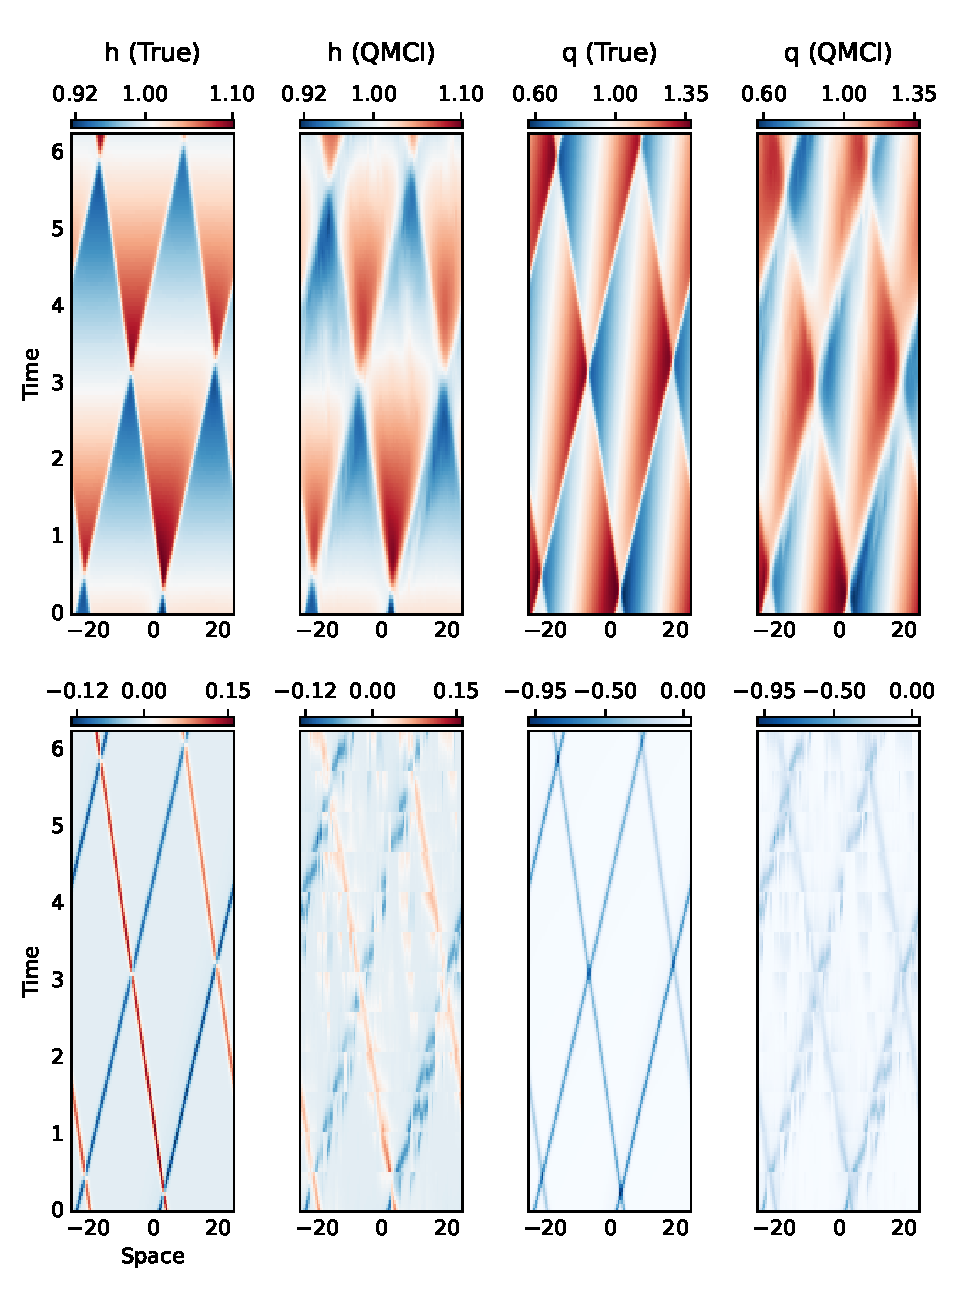
\includegraphics[width=.7\textwidth]{res02a.pdf}
    \caption{Space-time heatmaps for the trajectory with $\delta=0.75$.
    The layout of the plots is as in Figure \ref{fig:res01a}.}
    \label{fig:res02a}
\end{figure}

The results comparing the evolution under the true and surrogate
dynamics are grouped into four figures.
Figures \ref{fig:res01a} and \ref{fig:res01b}
include the results for the trajectory generated by the initial
condition obtained from
\eqref{eq:ic-family} for $\delta=0.25$.
Figures \ref{fig:res02a} and \ref{fig:res02b}
showcase the results obtained for $\delta=0.75$.

\begin{figure}[t]
    \centering
    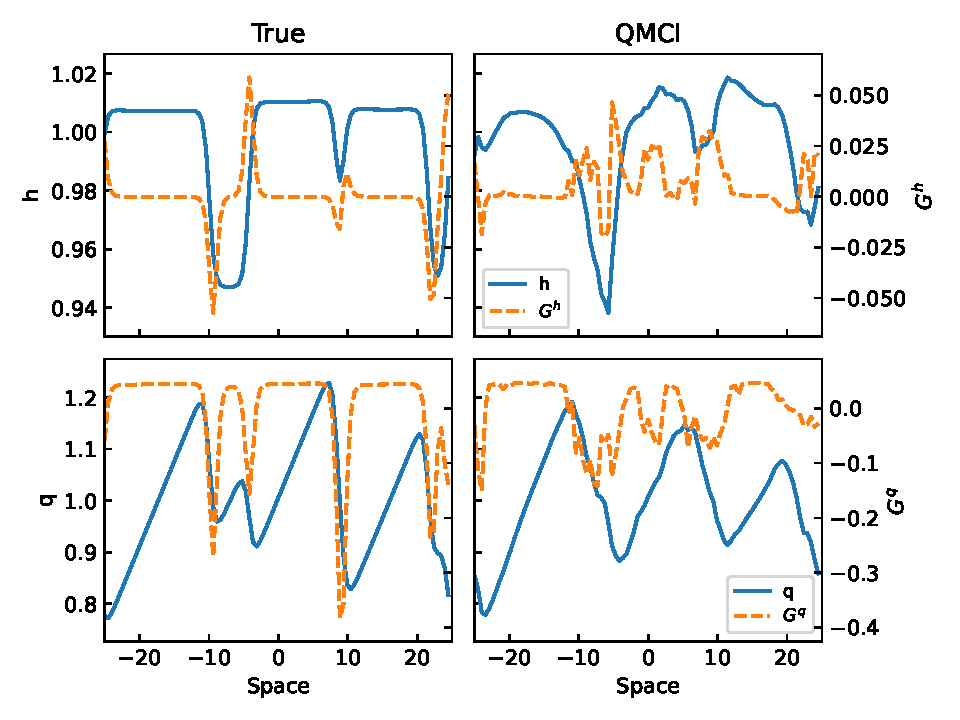
\includegraphics[width=.7\textwidth]{res01b.pdf}
    \caption{Spatial profiles of the final solution snapshot
    for the trajectory with $\delta=0.25$.
    The top row shows the results for the resolved state and the
    subgrid fluxes for the height field $h$;
    the bottom row for the momentum field $q$.
    In each row, the true results are on the left subplot,
    the predicted ones on the right subplot.
    Within each subplot, full lines are used for the resolved state
    with their numerical values indicated on the left axis;
    dashed lines are used for the corresponding fluxes with their
    values indicated on the right axis.}
    \label{fig:res01b}
\end{figure}

\begin{figure}[t]
    \centering
    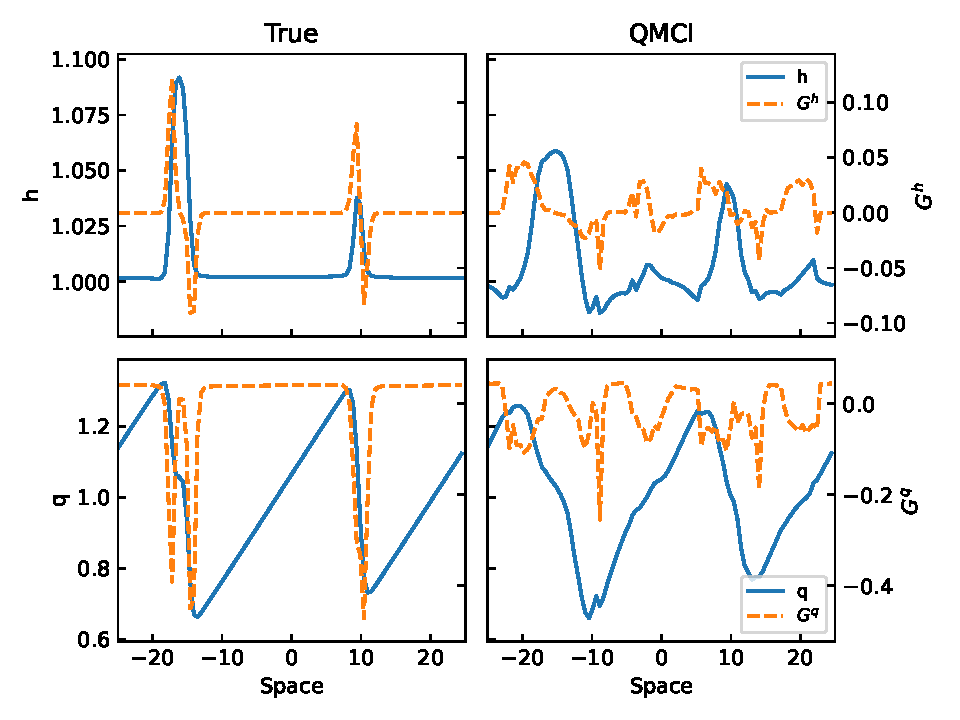
\includegraphics[width=.7\textwidth]{res02b.pdf}
    \caption{Spatial profiles of the final solution snapshot
    for the trajectory with $\delta=0.75$.
    The layout of the plots is as in Figure \ref{fig:res01b}.}
    \label{fig:res02b}
\end{figure}

\begin{figure}[t]
    \centering
    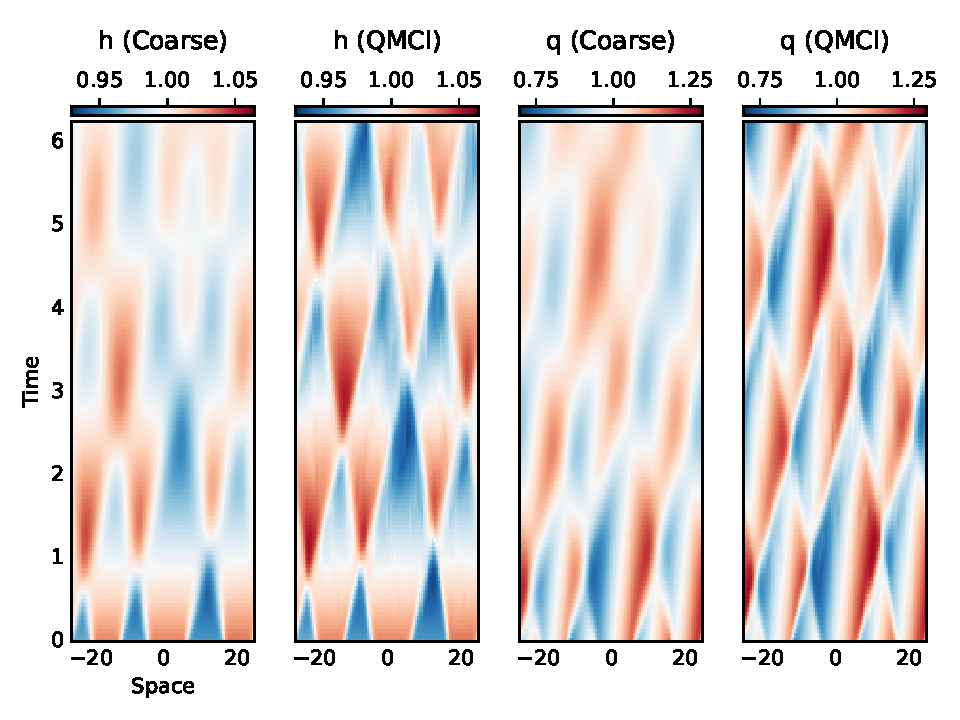
\includegraphics[width=.7\textwidth]{res01c.pdf}
    \caption{Space-time heatmaps for the trajectory with $\delta=0.25$
    comparing the dynamics on the coarse grid with the surrogate
    dynamics obtained by QMCl.
    From left to right, the first two plots show the results
    for the height field $h$, with the coarse grid results on the
    left and the QMCl results on the right;
    the next two plots show the results for the momentum field $q$,
    with coarse grid results on the left and QMCl on the right.
    The colorbars for each subplot are as in Figure \ref{fig:res01a}.}
    \label{fig:res01c}
\end{figure}

Looking at the heatmaps for the height and momentum fields in
Figure \ref{fig:res01a} for the trajectory with $\delta=0.25$
and in Figure \ref{fig:res02a} for the one with $\delta=0.75$,
we see that QMCl clearly captures the main features of the
dynamics for the tested time horizon.
For both trajectories QMCl correctly predicts the main
traveling wave features of the dynamics, including the spatial
variations of the waves as they interact with one another.
Moreover, the magnitude of the predicted fields is consistent
with the true dynamics in most regions of the spatial domain.
In addition to the results shown in these figures, we have
also verified that QMCl can reproduce the dynamical trajectories
included in its training dataset with good accuracy.

In the present closure model the subgrid fluxes play the role of
antidiffusive corrections to the fluxes generated entirely on the
coarse grid \cite{Timofeyev2025}.
Their values are proportional to the spatial derivative of the associated
field, taking large values when the height or momentum field is changing
rapidly in space, and approximately zero value when the fields are
constant in space.
As a result, the contribution of the subgrid fluxes is critical in regions
of large spatial variation of the height and momentum fields,
counterbalancing the increased diffusion of the solution introduced by our
coarsening of the original dynamics by spatial averaging.
The strong spatial variation of the true subgrid fluxes renders the
considered dynamics challenging to resolve and predict accurately
by any closure scheme
(Section \ref{sec:results-discussion}).
Typically, when the exact value of the subgrid fluxes is not
predicted correctly by the employed closure model
(derived by QMCl or another method),
the surrogate evolution will be more diffusive than the true
evolution.

The effect of diffusion can be seen in the heatmaps for the
two trajectories.
By comparing the true and predicted fields of height and momentum,
we see that the surrogate dynamics leads to stronger diffusion of
the solution in areas where there is strong spatial variation.
The increased diffusion is seen in the plots as bleeding of color
between different space-time regions, with the boundaries between
those regions being less sharp than in the true dynamics.
Similarly, the same effect can be seen by comparing the subgrid flux
fields for height and momentum.
In the true dynamics, the peaks of the fluxes are sharp and clearly
separated from the valleys, with clearly visible waves traveling in
opposite directions.
In the predicted dynamics, although the waves are still predicted
correctly, their peaks are not as sharp, with their values
diffusing more strongly to the surrounding region.

The flux plots also clearly demonstrate the effect of bayesian
conditioning, which for these results is performed every
$10$ timesteps ($\approx 0.5$ time units).
One can see the discontinuities that occur every $10$ timesteps
for the predicted fluxes over large regions of the spatial domain.
These discontinuities represent corrections introduced to the predicted
flux values every time conditioning of the quantum states is performed.
We perform the bayesian conditioning every $10$
timesteps to reduce the computational cost of the simulation,
since the conditioning is one of the most expensive operations
in our closure scheme
(Section \ref{sec:results-discussion}).
In general, the prediction accuracy
increases with increased conditioning frequency.
Based on our numerical experiments,
conditioning the quantum states every $10$ timesteps
strikes a good balance between prediction accuracy
and computational cost for the considered dynamics.

Similar conclusions can be drawn from the spatial profiles shown in
Figure \ref{fig:res01b} for the trajectory with $\delta=0.25$
and Figure \ref{fig:res02b} for that with $\delta=0.75$.
In these plots one can see that the subgrid fluxes are proportional
to the spatial derivative of the associated field, leading to sharp
variations in space.
The predicted dynamics preserves the main features of the evolved
fields, but struggles to capture the sharp peaks of the
subgrid fluxes, leading to stronger diffusion of the height and momentum
fields in regions of strong spatial variation.

To further demonstrate the crucial role played by the subgrid
fluxes in counterbalancing diffusion,
in Figure \ref{fig:res01c}
we compare the evolution of the QMCl surrogate dynamics
with the true dynamics generated entirely on the coarse grid,
namely with the subgrid fluxes
\eqref{eq:subgrid-flux}
set to zero at every grid point.
The comparison is carried out for the trajectory generated from
the initial condition \eqref{eq:ic-family}
with $\delta=0.25$
(Figures \ref{fig:res01a} and \ref{fig:res01b}),
but similar conclusions can be drawn from other initial conditions.
The comparison demonstrates that the surrogate fluxes predicted
by QMCl successfully counteract the diffusive effect of the
spatial coarsening seen in the coarse grid simulation
for the tested time horizon.
Namely, although the subgrid fluxes predicted by QMCl are not as
accurate as the true subgrid fluxes in regions of strong spatial
variation of the solution, they are nevertheless effective
in counterbalancing diffusion and thus improving the accuracy
of the predicted dynamics.


\subsection{Discussion}\label{sec:results-discussion}
In the following paragraphs we discuss several aspects of
the presented closure scheme and how they inform future
research directions.

\subsubsection*{Computational aspects}
Extending the QMCl framework to spatiotemporal dynamics comes with the
challenge of increased computational cost for its implementation,
primarily due to the increased size of the training datasets required
to capture the main features of dynamics that evolves over both space
and time.
As such, one key area of focus for future work is reducing the cost
of the numerical implementation of QMCl and improving its scaling
with sampling parameter $N$, spatial grid size $M$
and spectral resolution parameter $L$.

In the offline stage the most expensive operation is computing the
leading $L$ eigenfunctions of the $NM\times NM$ symmetric kernel
matrix $\matr{K}_N$ representing the kernel integral operator
\eqref{eq:data-integral-op}.
Even for moderate size parameters $N$ and $M$, solving such an
eigenvalue problem can quickly become very expensive.
As explained in Section \ref{sec:numerics}, to reduce this
computational cost when generating our numerical results
we performed a partial Cholesky factorization of
$\matr{K}_N$ to approximate it by a lower rank matrix
using the randomized numerical algorithm developed in
\cite{YChen2024}.
We then used the approximate kernel matrix to perform
its bistochastic normalization and solve the resulting
eigenvalue problem with reduced cost
\cite{Vales2025evd}.

As an alternative we also tried using the random Fourier
features (RFF) method to approximate $\matr{K}_N$
by a lower rank matrix \cite{Rahimi2007}.
However, we found that a relatively large number of Fourier
features was required to obtain a satisfactory approximation
of kernel matrix $\matr{K}_N$ compared to the rank
parameter $r$ required for the partial Cholesky factorization.
The poor approximations obtained using the RFF method led to
issues in the downstream bistochastic normalization of
the approximate kernel matrix,
often encountering negative or zero row sums that
prevented its normalization.
In addition to our empirical results, the difference in the
accuracy of approximations obtained using partial Cholesky
and RFF is also supported by the slower convergence rate
of the RFF method \cite{YChen2024}.
We intend to continue investigating effective ways of reducing
the cost of computing the kernel eigenfunction basis.

In the online stage the most expensive operation is the quantum
state conditioning; more specifically, building the quantum effect
operator from the current resolved state.
To form the quantum effect operator we use kernel
\eqref{eq:data-kernel-cond}
to compare the current resolved state vector to all state
vectors present in our training dataset.
This is the only online operation that scales with the size
of the training dataset $NM$, and requires that we have the
training data loaded in memory throughout the online stage.

One way of alleviating this issue is to use the RFF method
to approximate the out of sample evaluation of kernel
\eqref{eq:data-kernel-cond},
thereby eliminating the dependence on the training data
\cite{Rahimi2007,Giannakis2023}.
In our case this approach requires keeping in memory one
$L\times L$ matrix for each random Fourier feature used.
Namely, using $r$ Fourier features requires holding in memory
$rL^2$ floating point numbers of the employed precision.
In our experiments we found that a large number of Fourier
features was required to resolve the fine spatial features of
the state vectors, rendering this memory cost requirement
unsustainable.

Another approach is to form a reduced representation of the
training dataset and use that to form the quantum effect
operator.
For instance one could choose a subset of the original
training dataset and rely only on that subset to
perform the quantum state conditioning.
The formation of that subset can be carried out using the kernel
sampling algorithm that underlies the partial Cholesky factorization
algorithms \cite{YChen2024}.
Our goal is to continue investigating these and similar directions
for improving the performance of the quantum state conditioning
operation.

In QMCl the surrogate fluxes are computed as the expected value
of an observable with respect to a given quantum state.
As a result, to compute fluxes that vary strongly over the
spatial domain one has to ensure that the used quantum states
are very \emph{sharp}: obtaining a clear maximum in some
regions of product space $\Omega$ and being close to zero
everywhere else, formally similar to a finite sum of Dirac
delta measures.
Working with such sharp quantum states poses several numerical
challenges.

Producing accurate but very sharp quantum states requires
a very precise choice of bandwidth parameter $\epsilon'$
used in kernel \eqref{eq:data-kernel-cond}
for the bayesian conditioning.
Having such a selective kernel means that the resulting
quantum state leads to highly accurate fluxes when the correct part of
the training dataset is identified as similar to the current resolved
state.
However, it can lead to strongly inaccurate fluxes when regions of the
training dataset are misidentified as similar, compared to using a less
selective kernel that leads to wider averaging of the employed
quantum observable.

Moreover, the renormalization of the quantum state after
its bayesian conditioning can become a source of numerical
instability when working with a very selective kernel.
This can occur when no part of the training dataset
is identified by the conditioning kernel as being similar to the
current resolved state, leading to an approximately zero
feature vector and conditioned state.
More generally, obtaining an approximately zero conditioned
quantum state can happen when the prior quantum state and
the observation encoded in the feature vector have disjoint
supports.
In those cases, attempting to normalize the quantum state to
unit norm can yield unpredictable results.
Working with a wider, less selective kernel makes this scenario less
likely to occur, albeit with the tradeoff of less informative
conditioning and thus less accurate predicted fluxes.

Another way of addressing this issue is resetting the
prior quantum state to an uninformative state and repeating
the conditioning operation.
This requires erasing the historical information accumulated
in the prior state, thereby placing a higher level of
trust on the dynamical relevance of the observation.
Building a better theoretical understanding of the conditions
under which such a scenario might occur and the computational
ways in which it can be addressed is a topic of future work.

In addition to numerical instability, even if a very sharp quantum
state can be consistently obtained by using a very selective kernel,
there still remains the challenge of representing this quantum state
with respect to the eigenfunction basis.
Resolving such fine features usually requires a large number of
eigenfunctions, leading to expensive simulations.
Given that most QMCl operators are represented numerically as
$L\times L$ matrices, the overall simulation cost scales with
$L^2$.

The challenges involved in producing and working with a very
selective kernel function motivate our use of a kernel
bandwidth tuning algorithm \cite{Coifman2008}
and of the introduction of variable bandwidth
\cite{Berry2016,Giannakis2019acha}.
These measures help us define a kernel function that is
tailored to the characteristics of our training dataset,
which in turn allows us to strike a reasonable
compromise between numerical stability and sharpness
of the kernel used for bayesian conditioning.
As a result, we are able to construct a closure scheme
that can predict the main features of the considered
dynamics with reasonable computational cost and without
numerical instabilities.

Finally, the successful application of QMCl relies on the
precise calibration of kernel bandwidth $\epsilon$,
number of delays $Q$ and conditioning stencil size $J$.
Having efficient, reliable algorithms for selecting these
parameters based on a training dataset is very important.
The tuning of bandwidth parameter $\epsilon$ can be achieved
using the algorithm developed in \cite{Coifman2008}
or the median rule studied in \cite{Garreau2018}.
When applicable, choosing the number of delays $Q$
can be informed by the dimension of the attracting state space
region sampled by the dynamical trajectories generating the
training data \cite{Sauer1991}.
However, such dimension estimates are rarely available for
real world datasets and their underlying dynamics.
It would be interesting to consider computational algorithms
that can estimate a suitable range of values for $Q$ based
on the given training dataset, potentially also accounting
for the presence of noise
\cite{Zbilut1992,Marwan2007,Botvinick2024}.

\subsubsection*{Theoretical aspects}
One of the distinguishing features of the QMCl framework is that
the classical dynamics is first embedded into the noncommutative
setting of operator algebras used in quantum mechanics
and only then discretized to finite dimension.
Namely, instead of directly discretizing functions on
Hilbert space $H$ to obtain functions on finite dimensional
subspace $H^L$
we first map functions on $H$ to operators in $B(H)$
and then discretize them to obtain operators in finite
dimensional $B(H^L)$.
This process renders the discretization employed by QMCl
positivity preserving, with positive classical observables
and probability density functions mapped to positive
operators \cite{Freeman2024}.

In addition to structure preserving properties, this discretization
process embeds the discretized quantities in a space of larger
dimension than direct discretization.
More specifically, direct discretization maps real functions
on $H$ to functions on the $L$-dimensional subspace $H^L$.
The QMCl discretization maps real functions on $H$ to selfadjoint
real operators in $B(H^L)$ which is a subspace of dimension
$\frac{1}{2}L(L+1)$.
It is interesting to explore whether this difference
in dimension along with the noncommutative nature of $B(H^L)$
allow QMCl to encode more information about the original
dynamics compared to closure schemes performed in $H^L$.
Using tools from control theory \cite{Sontag1998}
and quantum information theory \cite{Nielsen2010}
one should be able to quantify the differences between the
two discretization approaches and their consequences
for downstream closure schemes.

Another question concerns the out of sample performance of QMCl.
In Sections \ref{sec:multitrajectory} and \ref{sec:numerics}
we considered training data generated by a finite collection of
initial conditions without reference to an explicit process of
generating these initial conditions.
A natural extension of this scenario is to consider an invariant
measure $\mu$ admitting a disintegration into conditional measures
$\mu_i$ sampled from a probability distribution of initial
conditions.
Interesting questions in this direction are to characterize
the behavior of our closure scheme as the number of sampled
trajectories increases and derive associated out of sample
error bounds.


\section{Conclusion}\label{sec:conclusion}
We have developed a framework for the dynamical closure of
spatiotemporal dynamics which combines elements of
the quantum mechanical closure (QMCl) framework developed in
\cite{Giannakis2019pre,Freeman2023,Freeman2024}
and the vector valued spectral analysis (VSA) technique of
\cite{Giannakis2019vsa}.
A key element of the present extended framework is that it
encodes statistical information about unresolved degrees of
freedom in the form of a field of quantum density operators
on the spatial domain.
This results in a flexible architecture where density operators are
collocated with the discretization cells of the coarse model
for the resolved dynamics.
The density operators communicate with the resolved dynamics by
providing the required flux terms through expectations of quantum
observables and by receiving information through operator valued
feature maps.
Moreover, our approach inherits the
symmetry factorization properties of VSA during the basis
construction process and can also be used with training data
consisting of multiple dynamical trajectories.
As with the original QMCl work, the process of embedding
classical dynamics into the noncommutative setting of quantum mechanics
leads to positivity preserving discretizations of classical observables
and probability density functions.

We have applied QMCl to a closure problem for the shallow water
equations on a periodic one dimensional domain.
The numerical results demonstrate that QMCl can effectively
predict the dynamics of the out of sample initial conditions
tested in this work, generating height and momentum fields that
agree both qualitatively and quantitatively with the true
data.
As expected from a dynamical system that demonstrates strong
spatial variations in the subgrid fluxes, the surrogate dynamics is
more diffusive than the true dynamics generated by a high
resolution reference model,
and eventually struggles to fully capture the sharp spatial features
of the true solution.

With that said, we believe that the results act as a successful proof of
concept for the extension of QMCl to spatiotemporal dynamics,
especially given the modest amount of data used for its training.
Everything else kept the same, we expect that increasing the
size of the training dataset $N$ or the spectral resolution $L$
will lead to improved prediction accuracy.

Future research directions stemming from this work include
improving the computational cost of the data driven implementation
of QMCl (particularly the cost of quantum state conditioning in the
online stage), as well as the development of strategies for
sampling initial conditions in the training stage and
kernel tuning/learning.
Additionally, we plan to explore applications of QMCl to systems
exhibiting spatiotemporal chaos.


\section*{Acknowledgements}
DG and JS acknowledge support from the U.S.
Department of Energy under grant DE-SC0025101.
CV was supported as a postdoctoral researcher from this grant.
DG acknowledges support from the U.S. Department of Defense,
Basic Research Office under Vannevar Bush Faculty Fellowship
grant N00014-21-1-2946.
DCF was supported as a PhD student from this grant.
We thank Ilon Joseph, Michael Montgomery and Ilya Timofeyev
for helpful conversations on the topics of this work.

\appendix
\section{Data driven implementation}\label{app:implementation}
The process of building and using the developed QMCl scheme to simulate
the surrogate dynamics consists of two stages:
the offline and online stages.
Below we outline the steps followed in each stage.

\subsubsection*{Offline stage}
The offline stage consists of the operations needed to build the
QMCl scheme using the training data
$\{\hat{x}_n\}_{n=0}^{N-1}$ and
$\{z(x_n,\cdot)\}_{n=0}^{N-1}$.
This involves the following sequence of steps.
\begin{enumerate}
\item Using the resolved state samples $\{\hat{x}_n\}_{n=0}^{N-1}$
we calibrate the bandwidth parameter $\epsilon$
for kernel \eqref{eq:data-kernel}
and perform its bistochastic normalization.
\item We use the samples $\{\hat{x}_n\}_{n=0}^{N-1}$
to compute the leading $L$ eigenfunctions
$\{\phi_\ell\}_{\ell=0}^{L-1}$
of integral operator
\eqref{eq:data-integral-op},
defining subspace $H_{\Omega,N}^L$ as their linear span.
The eigenfunction basis is represented by matrix
$\matr{\Phi}\in\Rbb^{NM\times L}$
holding one eigenfunction in each column.
\item We form the transfer operator $P_N^L$
and represent it by matrix
$\matr{P}_N^L\in\Rbb^{L\times L}$.
\item We use the flux samples $\{z(x_n,\cdot)\}_{n=0}^{N-1}$
to form two quantum observables and project them to operators
$A_0$, $A_1\in B(H_{\Omega,N}^L)$
represented by the matrices
$\matr{A}_0$, $\matr{A}_1\in\Rbb^{L\times L}$.
The first observable is built using the flux samples
$\{z_0(x_n,\cdot)\}_{n=0}^{N-1}$
corresponding to the height $h$ variables;
the second using
$\{z_1(x_n,\cdot)\}_{n=0}^{N-1}$
corresponding to the $q$ variables.
\item We define the discrete field of quantum states
$\rho\in L^2(S,\nu_M; B(H_{\Omega,N}^L))$
with one state corresponding to each coarse grid cell.
Each quantum state
$\rho(s_m)\in Q(H_{\Omega,N}^L)\subset B(H_{\Omega,N}^L)$,
$s_m\in S_M$
is represented by a vector $\vect{\rho}_m\in\Rbb^L$.
\item Using the resolved state samples $\{\hat{x}_n\}_{n=0}^{N-1}$
we calibrate the bandwidth parameter $\epsilon'$
of kernel \eqref{eq:data-kernel-cond}
and compute the bandwidth function needed for its variable
bandwidth generalization.
\end{enumerate}

\subsubsection*{Online stage}
In the online stage we use the operators built in the offline stage
to timestep the surrogate dynamics.
We denote by $\tilde{x}\in\Xcal$
the resolved state predicted by QMCl to distinguish it
from the true resolved state $\hat{x}$.
The online stage consists of the following steps.
\begin{enumerate}
\item We initialize the resolved state $\tilde{x}$.
\item We initialize the quantum states $\rho$
representing each grid cell using an uninformative initial condition:
each quantum state $\rho(s_m)$ is set to the projection along the
unit function $1_\Omega\in H_{\Omega,N}^L$
that takes the value $1$ everywhere.
\item We condition each quantum state using the initial resolved state
$\tilde{x}$ and training data $\{\hat{x}_n\}_{n=0}^{N-1}$.
\item We use the quantum states $\rho$ and quantum observables
to compute the surrogate fluxes $\tilde{z}(\rho)$
corresponding to two flux values for each grid cell.
\item We begin the timestepping loop.
\begin{enumerate}
\item We update the resolved state $\tilde{x}$
using the surrogate fluxes.
\item We update the quantum states $\rho$ using the transfer operator.
\item We condition the quantum states using the updated resolved
state and training data samples.
\item We compute the updated surrogate fluxes $\tilde{z}(\rho)$.
\end{enumerate}
\end{enumerate}

In the timestepping loop as presented above, the quantum states
are conditioned at every timestep.
In our presented numerical results we have elected
to condition the states less frequently, by only performing
bayesian conditioning every $N_r$ timesteps with
parameter $N_r\in\Nbb$.

\bibliographystyle{elsarticle-num}
\biboptions{sort&compress}
\bibliography{refs}

\end{document}
